\documentclass[pdftex, 12pt, a4paper]{article}

\usepackage[pdftex]{graphicx}
\usepackage[utf8x]{inputenc}
\usepackage{appendix}
\usepackage{cite}
%\usepackage{pgfgantt}
%\usepackage{pst-gantt}
\usepackage{rotating}
\usepackage{pdflscape}
\usepackage{hyperref}
%\usepackage{breakurl}
\usepackage{listings}
\usepackage{nomencl}
\usepackage[a4paper]{geometry}
\usepackage{tabularx}
\usepackage{longtable}

\nomitemsep 1pt

\makenomenclature

\begin{document}

\begin{titlepage}

\begin{center}

{\large Electronics and Computer Science\\
Faculty of Physical and Applied Sciences\\
University of Southampton}\\[5em]

{\LARGE On the Implementation of Authentication Mechanisms for Mobile Devices over Wireless Networks}\\[5em]

{\large Thomas Grainger}\\[5em]

{\large \today}\\[5em]


\end{center}

\end{titlepage}


\begin{abstract}
The project sets out to determine if those who distribute malicious content
use trending topics on services such as Twitter or the News Media so as to
gain some of the traffic from users searching for legitimate information about
those topics.

The project discusses design and implementation of a distributed framework
designed to organise multiple subsystems that process trending topics from
these sources and emulate a user browsing for pages related to those trending
topics. In the process those pages accessed are evaluated for malicious
content hoping to distribute malware to unsuspecting users using drive by
download toolkits.

\end{abstract}

\tableofcontents
%acknowledgments
\section*{Acknowlegements}
\addcontentsline{toc}{section}{Acknowledgments}

Our customer Team Cymru and their representative Chas Tomlin.

The Celery community, in particular Ask Solem Hoel (@asksol) 

Proof Reading: Ali Emamy, Matthew Power, Chrissie Metcalf
%project description (problems + goals)
\section{Introduction}

%chris's intro stuff
\subsection{Emma Watson and Malware}
On September 10th 2012, MacAfee released a report detailing a list of the top 20
celebrities that it believed were the most risky to search for on the internet\cite{mac-watson}.
The report specifies a number of threats from risky web sites, such as malware,
phishing, and spam, and determined that Emma Watson was the most risky celebrity
to search for on the web with more than 12.6\% chance of a site being malicious
when searching for her name combined with phrases such as ``free download''.

The hypothesis suggested in the MacAfee report is that trending topics have
malicious web pages crafted specifically to target the topic, and this is the
hypothesis that will be investigated in the project.

Before investigating if malware is targeted at trending topics, it is necessary to
investigate exactly what constitutes a trending topic. ``Trending topic'' is a term
that originates from Twitter, where statistics are collected on users tweeting
with a given hashtag and used to determine popular hashtags, presented in the
user interface a ``trending topic''. When discussing trending topics in this
report, other sources of trends and popular subjects will also be considered as
trending topics.

To make it possible to investigate the hypothesis proposed above a framework
will be designed and built to automatically gather trends, search for URLs
relating to the trends, and then attempt to detect whether the URL is hosting
malicious content. The data will then be collected into a database, allowing the
hypothesis to be tested. Results will be reported using a web interface that
will also be capable of monitoring the status of the malware scanning system.

%nafiseh's intro stuff
\subsection{Problem Definition}

\paragraph{} 
The continually increasing variety of known and unknown malwares make malware detection a difficult problem to solve. As malware detection systems become more intelligent and sophisticated, malware writers are also developing more advanced methods. Some anti-virus software is ineffective in terms of detecting unknown malware. This project seeks to design a malware detection system capable of identifying web pages containing malicious content for a given contextual topic as represented by trending search keywords. 

\paragraph{} 
Also, this research involved emulating a user browsing for these keywords. The challenging part of this project arose in seeking to define a malicious web page, as there are many variations of an infected webpage depending on the type of malware. 
Some types of malware directs the user to an illegal website by clicking on the URL. A large group of malware are designed with a commercial objective in mind. A webpage that has poor content, offers no goods or services and is used for the purpose of directing users to unsolicited advertisements is an example of commercial malware. Whilst other web pages may look perfectly fine at first glance but in fact contain malicious functions, for example by using JavaScript functions. In the case of the latter, the detection is even more difficult because the malware is a type of obfuscation malware that is hidden from the user. Moreover, malwares could come from a variety of different sources.
The examples above highlight the difficulties of this project. Furthermore, whilst a great deal of research has been performed on the subject of malware detection and the effectiveness of various detection methods, such research specifically considered a specifically defined type of malware and analysed the methods used for that particular malware. 

\paragraph{} 
In seeking to propose a malware detection system capable of identifying web pages containing malicious content based on trending search keywords, this paper gives consideration to the fact that different variations of malware exist. 


%literature review 
\section{Literature review}

Malware is now an international word, which gained prominence following the
creation and development of the internet. There are many definitions of
malware. Malware is often defined as a short form of malicious software 
containing malicious programs such as computer viruses and worms. With the
increasing sophistication of malware attacks and their potential for causing
major damage and disruption, there is an ongoing need for the development of
more advanced malware detectors\cite{Malware-tech}.

\subsection{Malware Detection: Approaches}

Malware detectors employ a variety of malware detection techniques depending on
the type of malware being targetted. In general, malware detection techniques
can be classified into two groups: the first group is heuristic-based (or
anomaly-based) detection that defines normal behaviour in order to determine
the maliciousness of the software. The second group is signature-based
detection that compares the code content to the code signature of known malware in
order to decide the maliciousness of a program under inspection. However,
current detection techniques that are based on known malware are unable to
detect a malcode unless it has been executed. Hence, not all malwares can
be detected by these two techniques alone. Therefore, it is crucial to consider how
we can extend the available detection tools by designing and developing a
detection system capable of detecting other unknown
malwares\cite{Malware-tech}.
 

In recent years, machine learning methods were introduced to the malware
detection systems to extend the effectiveness of heuristic-based methods. The
classification algorithm is one of the standard methods in machine learning
that could solve the problem of detecting unknown malwares\cite{Machin-learn}.
The idea of classification algorithm is based on pattern matching. The
classifier contains a set of learnt patterns and decides the maliciousness of
an unknown program by comparing to these learnt patterns. The learnt pattern set is as
a result of applying learning methods on a training set that contain instances
of both malicious and benign files. A recent study on integrating machine
learning methods with heuristic-base methods produced positive results in
detecting new malware\cite{Machin-learn}. The file representation and feature
selection methods are other machine learning techniques that greatly improve
the result of malware detection systems. The latter method is concerned with
patterns used for demonstrating executable files while the former seeks to
decrease the dimensionality of patterns that appear in the
file\cite{Machin-learn}.

Polymorphic viruses are a complex type of malware that many widely used malware
detection software will fail to detect because such malware detection software
tends to employ Heuristic-based and signature-based algorithms. Furthermore, the
drawbacks to using signature-based methods are that they are expensive and also
slow.  The recently designed system called Intelligent Malware Detection System
(IMDS) is capable of recognising both polymorphic and previously unseen
malicious executable (new) malware. The evaluation and experimental results of the IMDS illustrated its high performance compared with some anti-virus software such as McAfee virus scan. IMDS uses data mining based classification method and the architecture of the IMDS system includes three main modules; the parser,the rule generator and the malware detection part\cite{IMDS}.

One of the most commonly used formats for reading documents is PDF. Therefore,
it is likely that an attackers use PDF files for malicious purposes. Also, it
is important to note the structure of PDF documents, which is made up of a
sequence of flexible dictionary objects. This flexibility makes PDF files more
attractive for an attacker because they can host a variety of applications such
as java script and embedded files. Attackers mostly apply obfuscation
techniques to bypass intelligent detection systems. With the aid of machine
learning techniques, a new PDF detector has been designed to recognise infected
PDF documents\cite{maiorca2012pattern}.  The PDF detector contains three main
steps; a data retrieval module, a feature extractor module and the classifier.
The system adapted K-mean clustering method to collect the set of keywords for
the feature extractor module. The classifier was tested using different
classification algorithms such as Naïve Bayes and SVM, with the most accurate
and efficient algorithm being selected for the final
design\cite{maiorca2012pattern}.
 
The signature-based method can fail to detect the obfuscation code because the
obfuscation only has a minor effect on execution behaviour. Gao et al proposed
the semantic based malware detection algorithm to handle obfuscation in
infected documents. According to this algorithm the semantic of the program is
compared to the semantic of the malware. As a result, this proposed method
reduces the need for frequently updating the malware database; hence making it
remarkably robust\cite{Amom}. 


Malware is continuing to grow and become more complex. An effective malware
detector must be capable of detecting unknown malware as well as hidden
malcode. However, malware writers analyse the techniques used in commercial
malware scanners and attempt to produce new malware that can bypass the
techniques adopted by such virus scanners. Therefore, an increase in unknown
malware is, at present, innevitable\cite{vinod2009survey}.


Another study performed on malware detection methods was called BINSPECT, which
provided a lightweight approach to identifying malicious web pages. This
approach employed supervised learning technique for its detection and
considered malware distributing techniques such as; phishing,
derived-by-download and injection\cite{eshete2012binspect}.

BINSPECT used an unknown webpage as an input and classified the web page as
either malicious or benign. Its classification relied on the features extracted
from a given web page and the web page features were defined in three
categories; features of URL, source code of webpage and social reputation
features.  For the URL features, the structure of URL (for example, number of
dots ‘.’) or the length of the URL string was analyzed. The results showed the
most malicious URL had an abnormal length. For the web page source code, an
emulated browser was used to capture the obfuscated JavaScript. Some of the
features considered in the web page sources code included the number of; lines,
links and suspicious functions. The extracted features were then used to
collect the data for the training set and learning set. The data was then
classified by applying machine-learning methods such as Logistic Regression,
SVM (Support Vector Machine) and Decision Tree\cite{eshete2012binspect}.  The
paper concludes its proposed method is very effective in detecting a malicious
webpage with an accuracy rate exceeding 97\% and that by adding the new
features to the system improved its performance significantly. However
BINSPECT lacked the ability to analyse obfuscated
JavaScript\cite{eshete2012binspect}. 


%Previous reports in the relevant areas were researched. In this section we are
%going to introduce some background knowledges and research contributions
%summarised from three reports written by authoritative institutions. We will
%see the importance of trending keywords in malware distribution, and the
%methods and systems to measure and counter them. Approaches for malicious
%website detection and analysis are also included. 

\subsection{Search-engine optimization} 

Search engine is a key tool for
exploring resources on the Internet and becomes increasingly significant in
people's daily life. Many famous search engines index web pages are using PageRank
algorithm, which states that the rank of a web page depends on the quantity and
quality of incoming links, and the higher is the rank, the more likely that the
web page will appear in the top results of a search query. Although search
engine providers do not usually reveal their algorithms in calculating
PageRanks in order to reduce spammers who gaming with the system, many main
features are still well-known. For example, many web pages have their main title
stored in the URLs, therefore the URLs themselves may represent a summary of the
page contents, which is a feature that can be utilised by website administrators 
to rise PageRank.
\paragraph{}
A report produced by University of Washington and Microsoft
Research Silicon Valley introduces a widely used search results poisoning
technique named Search Engine Optimization (SEO) as well as a system that
automatically detects them, called deSEO.\cite{deseo} They claim to be "the
first to present a systematic study of search-result poisoning attacks and how
to detect them". SEO is a process that uses varies approaches to affect a web
page such that it will appear in higher positions of a search engine's search
results, and for most of the cases, a rise of PageRank is achieved. This
process can be exploited to support illegal websites, such as malicious
websites, with some additional unethical techniques (which will be introduced
later) therefore achieves conspicuous boosts in PageRanks. This is called SEO
attacks. According to the paper, a typical SEO attack consists three servers,
which are compromised server, redirection server and exploit server. The
process of exploitation can be divided into five steps: 
\begin{enumerate} 
\item The victim submit a common request to a search engine.
\item The victim click on a search result and is navigated to a malicious web
page hosted on a compromised server.
\item The compromised server forwards the request to a redirection server.
\item The redirect server selects an exploit server then navigates the user
to it. 
\item Exploitation of the victim's browser or scareware displayed. 
\end{enumerate}
\paragraph{}
To compromise a server, the attackers often target specific popular software
with known vulnerabilities but are still used by many servers. The example in
the report is a shopping websites management software called osCommerce, and
the attackers compromise the servers by uploading PHP scripts. Those scripts
are likely to have functions that can navigate through the server's file system,
find data, and upload further files etc. When a server is compromised, SEO
pages can then be generated. Those pages contains a large number of links
connects to other SEO pages (probably on other compromised servers), as well as
contents that relate to the keywords this page's URL focuses on. Such dense
link structure and high relevant contents are the main means to elevate the
PageRank. The generated SEO pages may have clocking techniques, which means
they present different contents to search engine crawlers and victims. When the
page is visited by a search engine crawler, links to other SEO pages and
poisoned keywords are displayed, and when a victim accesses, the user's browser
is forwarded to a redirection server. 
\paragraph{}
Redirection servers are often formed
with several layers before reaching the exploit server, where they redirect
within the compromised server network. In the paper's case the domains of those
servers are very similar, and according to their IPs it is determined that those
servers are hosted in physical groups. The Exploit servers in that example have
191 domains being hosted on only two IPs, and the web page is very cautious with
incoming visitors. The page detects search engine crawlers as well as referrer,
and also blocks IPs from search engine companies. 
\paragraph{} 
The
researchers of the report crawled across the network of SEO links and finally
determined 5400 compromised domains. Each domain have an average links of
80,000 to other domains with 8,000 keywords corresponding to the same number of
SEO pages, which proves the use of dense link structure in rising PageRank. 
They also provided an estimation of the number of victims affected by this
group of domains, which was produced from a dataset collected for two and a
half months. The conclusion was that over 81,000 users were directed to exploit
pages.
\paragraph{} 
The detection of SEO attacks is not a trivial task, as
those pages usually trigger malicious actions only after strict requirements
are met, such as depending on the execution result of a JavaScript with the
input of a user's mouse action. Fortunately the report proved that studying only
the URLs' structures is sufficient to complete the detections. 
\subsection{Trending-term exploitation}
Beside from how a SEO attack is technically implemented, the kind 
of websites that apply SEO and the ways they are found by victims are researched. SEO is a 
process of improving PageRank, and before a web page's PageRank is taken into 
account in a search query, their content must match with the keywords of the query. Many
well-known public websites and search engines provide trending data in real
time (such as Google Trends and Twitter Trends), therefore the easiest method to
determine what people are searching is to collect trending keywords/terms. With
trending terms the web page's contents are then usually generated by sending
search queries with those terms, and combine contents in the URLs returned.
\paragraph{}
In this section a new report focuses on researching ad-filled and malicious
websites.\cite{moore2011fashion} It claims to be the "first large-scale measurement
and analysis of trending-term exploitation on the web", and as a result they
concluded the ways of trending terms application in spam among the web, with a
huge dataset collected through nine months containing over 60 million search
results. The report includes a wide research from trending terms collection to 
economics analysis, however here only topics relevant to the 
project are introduced. 
\subsubsection{Data collection and classification}
A trending terms dataset is categorised into trending set and control set. 
Trending set is formed by fast-changing popular terms, obtained from Google 
Hot Trends. These terms will become ``cooled'' in near future and are dropped 
from the dataset if so. Control set consists constantly popular search 
keywords, with the purpose to find out any "phenomena unique to the trending 
nature".\cite{moore2011fashion} The terms are then automatically fed to search-engines with optimised 
time interval. According to their experiments, 85\% of results are identical 
when comparing the results obtained from tests with 10 minutes and 4 hours 
intervals, and finally the 4 hours interval is applied to all their programs. Top 
results of each search query are stored in the dataset for classification, 
where in their case 32 results from Google and 100 results from Yahoo! are used.
\paragraph{}
In the report they organise websites into three categories, benign, 
malware-distributing and ad-filled, where ad-filled sites are also called Made 
for AdSense (MFA). For malware-distributing sites they simply check them with 
Google Safe Browsing API, in contrast for MFA sites they developed a 
supervised machine-learning algorithm then completed it with 363 manually 
inspected MFA sites as training set. As a result, for all URLs collected, 
0.30\% terms from the trending set and 0.13\% terms from the control set are determined to 
have malware and 6.2\% keywords from the trending set are MFA sites. 
\subsubsection{Measurement of trending-term abuse}
This report referred number of times to John et al.\cite{deseo}, which was 
reviewed in the previous section. The authors confirmed dense link structures in 
both MFA and malware-serving websites. For MFA sites they built a directed 
graph and proved the existence of a ``fairly large, collusive MFA operation'' 
who owns 30.7\% of all MFA sites, while for malware-serving websites, as 
reported in the previous section, they found that a large portion of 
compromised servers are controlled by a single group, named a campaign. The 
same pattern appears in Twitter posts containing MFA links. Their data 
illustrates that 50\% of the MFA tweets direct to only 7.2\% of MFA domains 
across all MFA domains involved in Twitter. 
\paragraph{}
The authors then carried out a research in examining characteristics of 
trending terms. They classify trending keywords with Google Insights for 
Search, then find out the peak popularity estimate and advertising value 
provided by Traffic Estimator for each keyword. An observation is that all 
categories of keywords are targeted by malware and MFA, however the 
distribution of malicious sites varies according to a keyword's popularity and 
advertising value. More specifically, referring to their data, the percentages 
of malware-distribution and MFA sites decrease as the keyword's peak 
popularity and advertising value rises. They also conclude that, as a source 
of revenue, "malware and MFA behave more like substitutes, rather than 
complements".\cite{moore2011fashion}
\subsubsection{Search-engine intervention}
Google stated some modifications of its search-engine ranking algorithm in 
response of increasing SEO behaviours on 24th February, 2011. As the date was 
between their project's data collection duration, the report includes an 
investigation of the effectiveness about this announcement. \\
They compared the percentage of MFA sites in top 10 search results, with the 
conclusion states a decrease from 3.1\% to 0.47\% after a month later to the 
announcement date. They also collected the number of visits to MFA sites, 
which proved that the visits to MFA sites using Google ads had been decreased 
by 41\%, where those without had a reduction of 93\%. 
\subsection{Automatic malware collection}
The most popular means to distribute malware (SEO) is introduced, 
with trending terms as a significant role. In this section we will know the 
methods to detect malicious websites and analysis malwares in them, and 
finally collects malicious code across the web. A report carried out by Korea 
Internet \& Security Agency\cite{automalwarecollecting} explained a system 
that collects malicious code from malware-distributing websites found by 
search-engine with trending keywords. The report presents three approaches 
categorised into active and passive for detecting whether a website is 
malicious: 
\begin{enumerate}
\item 
{\bf Passive Malware Detection}\\
In this method the attackers are allowed to infest the system, then local analysis 
is performed with the malware. Server honeypot is an example of this approach, which hosts 
a vulnerable system and waits for exploitation. 
\item
{\bf Active Low Interaction Client Honeypot}\\
In this case the malicious website is accessed, with only HTML downloaded 
however not executed. Static analysis is then applied to the file. The main 
advantage of this approach is simplicity. This kind of honeypots require 
minimal resources to maintain and employ while does not give visible 
risks.\cite{honeypots}
However limitation exists. The most obvious point is this kind of systems are 
designed to detect known threats, because there is no way to find out the 
behaviours of a new type of attack without executing them. Another problem is 
that it is impossible to check the contents of a page if it contains interactive 
scripts which cannot be downloaded. For example, a block of script may require 
sources from other files, which cannot be examined further without running it. 
\item
{\bf Active High Interaction Client Honeypot}\\
The term high interaction means the malicious web page is actually visited by a 
real browser under a real vulnerable system. 
The file system and registry are then scanned for modification. This approach 
requires a light-weight operating system which can be reset without 
significant time cost. An obvious advantage is that a thorough test can be 
performed to avoid any dynamic content cannot be found by static analysis, 
which means further amount of information includes the 
full behaviour of an attack can be collected. Another point is that the high interaction system 
does not predict how the attack will behave, instead it gives an open 
environment which monitors all activities.\cite{honeypots}
However it is still not perfect, as some malicious code may require specific 
environment in order to execute, such as a certain version of browser and 
operation system combination. The system also requires significantly more 
resources than low interaction methods, including memory, disk space and 
computing power. 
\end{enumerate} 
The two active methods can be combined to overcome their shortages, which 
creates a new hybrid method. 
\paragraph{}
In the report they implemented an automated malware collecting system 
utilises both low and high interaction approaches. The overall execution flow 
of their system is as following:
\begin{enumerate}
\item Trending keywords (or ``search keyword that reflects the social issue'' 
as the report said) are collected from various search engines. Though details 
in this step is not described in the report. 
\item Search queries are sent with those trending terms to a number of search 
engines. The top URLs returned are stored in a URL dataset. 
\item A URL component check is performed as a low interaction detecting 
method. For each URL they download and crawl the web page to find out any 
suspicious behaviours. The checked criteria include the existence of zero 
size iFrame, the intensity of obfuscated scripts, frequency of \% symbol and 
frequency of particular function calls. They discovered that an 
obfuscated JavaScript in a malicious web page usually contains significantly 
longer unique character streams, and similar patterns occur for \% symbol 
frequency and function calls. In the end they concluded a term called web page 
entropy which sums all the features described above, that can then be used to 
classify whether a web page is malicious or not. 
\item Web pages recognised as malicious are sent to a high interaction client 
honeypot which automatically visits the page and collects malicious code 
distributed. They utilise a single virtual machine with the most vulnerable 
environment, however details about the environment are not included. They 
isolate newly created files and prevent their execution while also normalise 
any obfuscated scripts downloaded. 
\end{enumerate} 
\paragraph{}
In the performance verification section a comparison of 
their system and other existing active malware detection systems (HoneyMonkey, 
HoneyClient and MonkeySpider) shows that the new hybrid one has significant 
advantages in static analysis, false positive rate and system recovery speed. 
It is also the only system that is able to recover obfuscated script and 
pre-process URLs. 
\paragraph{}
Their data collection period spans for one and a half month, resulting 1287 
unique suspicious file collected. They test these files in two steps: first 
scan them with commercial anti-virus software, four vaccine programs were used 
in their case, then for the remaining non-virus files they send them to 
behaviour analysis systems such as ThreatExpert and Norman SandBox. As a result 
a total of 986 are determined to be malicious, where 119 of them are only 
discovered by behaviour analysis systems. 
The URLs are collected from search-engines, email spam and blacklists. 
Unfortunately the report does not include details about the source and 
quantity of their trending terms, and size of the URL dataset is also unknown. 


\subsection{Related work}

\paragraph{} 
Over the past few years, the internet has been used by an attacker to distribute a malware. Search engines can be used as a medium for spreading a malware through the internet. Essentially, attackers use the search engine optimisation algorithm applied by Google to insert their malicious links in the most visited websites. Based on deSEO observations, attackers used trendy keywords and regenerated relevant content pages in order to achieve a successful attack\cite{deseo}.

Therefore, a recent study has been undertaken to detect the malicious links based on such trendy keywords. In this study, the proposed detection method identifies suspicious websites by analysing the components of the URLs. In the second step, each suspicious websites is clustered based upon its lexical structures. Finally, a cluster analysis is undertaken in order to select the suspicious group\cite{deseo}.
The dataset required for this experiment was collected from Google and Bing search engines. The data set was divided into two groups, the first group was used for training and the second group was used for the purpose of learning. The system can automatically identify additional malicious URLs. However, detection will most probably fail if the attacker does not use the keyword in the URL\cite{deseo}.

\paragraph{} 
A recent study undertaken in 2011, analyzed the increasing amount of malware that related to the trendy-terms. This research provides the first large-scale measurements of using trending terms in web search engines over a period of nine months. This research how the attackers use trending keywords to direct users to advertising websites. These websites profit by displaying advertisements on their webpage without offering any goods or services\cite{moore2011fashion}.

The proposed methodology is based on data collection and website classification. The data for this study is collected from different sources such as Google, Bing and Twitter. The websites are classified into two groups, malicious and benign. The malicious websites can be a malware hosting website, or may contain advertisements\cite{moore2011fashion}.

According to this paper, their system added hot trendy topics to the list of trendy term every hour and removed older terms from the list after 14 days. The result of their measurements showed that a high percentage of the malware belonged to Google Hot trending topics. Also, the comparison between trendy terms and popular topics highlighted that both topics were valuable tools for attackers in distributing the malware. However, trendy terms returned a higher number of infected webpages. The difference being that a popular topic can last for a longer period of time and its related website always has visitors, whilst a trendy term will stay popular as a ‘hot topic’ for a short period of time and have a lot of visitors during that short time period\cite{moore2011fashion}.

%Specification + Customer Feedback (--> Design)
\section{Specification} To aid in the task of designing the solution, a set of
requirements have been drawn up. These requirements have been derived from the
division of the task presented in the goals of the project with MOSCOW priority
attached to each.

\begin{enumerate} \setlength{\itemsep}{1pt}
    \item The system \textbf{must} be able to collect trends.
    \item The system \textbf{should} be able to collect trends from more than once source.
    \item The system \textbf{must} be able to discover target web pages using a search engine .
    \item The system \textbf{should} be able to discover target web pages using multiple different search engines.
    \item The system \textbf{could} be able to discover target web pages using Twitter.
    \item The system \textbf{must} be able to determine if a page is malicious or not.
    \item The system \textbf{wont} detect ad-ware and made for ad-sense pages.
    \item The system \textbf{wont} detect Phishing.
    \item The system \textbf{must} be able to control multiple different malware scanning components.
    \item The system \textbf{must} use High Interaction malware Scanning.
    \item The system \textbf{must} use Zero Interaction malware Scanning.
    \item The system \textbf{must} use Low Interaction malware Scanning.
    \item The system \textbf{should} be able to dispatch dispatch only likely candidate malicious URLs to slower High Interaction Scanners.
    \item The system \textbf{should} be able to fine tune High Interaction Scanner dispatch probability.
    \item The system \textbf{could} use historical speed and current status of the system to influence High Interaction Scanner dispatch probability.
    \item The system \textbf{must} be able to store data determined about targets.
    \item The system \textbf{must} be able to relate data about targets to the
    trend source and time it was discovered on.
    \item The system \textbf{must} be able to generate reports.
    \item The system \textbf{should} be able to show the time taken for a particular.
    \item The system \textbf{could} display reports dynamically using a web based interface.
    \item The system \textbf{should} be able to monitor the status of the system.
    \item The system \textbf{should} be able to monitor the status of each malware scanning component.
    \item The system \textbf{could} be able to display statuses with a web interface.
\end{enumerate}

\section{Customer Interaction} The project was put forward by Team Cymru
Research NFP, ``a specialized Internet security research firm and 501(c)3
non-profit''\cite{team-cymru}. Team Cymru maintains various real-time monitoring
``pods'' to measure the status of malware on the public Internet. The project
compliments their existing offerings by incorporating social media and news
trends with active web scanning.

Over the course of the project the group had two meetings with Team Cymru
representative Chas Tomlin: a video conference and an informal meeting.
Meetings were intended to occur at the start of the project and after each of
the presentations, however only one of the post-presentation meetings occurred.

The video conference was used to introduce the group to Team Cymru and discuss
the project requirements, in which the brief was expanded upon. The
specification was influenced by requests to: 

\begin{enumerate}
    \item A requirement to emulate a user browsing the web using a virtualized
            web browser also referred to as High Interaction Malware Scanning.

    \item A requirement to use simple crawling and static analysis as in Low
        Interaction Malware Scanners, to be determined as part of the literature
        search.

    \item A suggestion to create a scanning modules that uses signature oriented
        scanning of pages and the hyper-linked files

    \item A suggestion to write modules that make use of existing repositories
        of malicious websites such as Google's Safe Browsing
        API\cite{google-safe} Google's Safe Browsing API and the crowd sourced
        Web Of Trust.

    \item Make the code machine-independant, so as to allow the scanning modules
        to operate on cheap, commodity, cloud machines such as Amazon Web
        Services Spot Instances\cite{aws-spot} or Rackspace Cloud
        instances\cite{rackspace}
\end{enumerate}

Also discussed was the possibility of downloading and investigating a ``Drive by
Download'' malicious software distribution tool.  The legal considerations of
downloading and executing an illegal piece of software are complex and as such
would require the group to obtain a detailed set of permissions before
attempting such a task.

While researching this as a possibility because of such considerations it was
determined that the time and effort required to obtain permissions to would be
prohibitive the decision was made to not investigate ``Drive By Download''
toolkits as part of the project.

After the first presentation an informal meeting was held to discuss progress on
the project so far with Chas:

\begin{enumerate} 
    \item A suggestion to use Internet Explorer 6 running under
            several interfaces of Wine to act as a faster High Interaction
            malware scanner than virtualizing an entire operating system.

    \item A suggestion to use ClamAV as the scanning engine behind the signature
        oriented scanning malware scanner.

    \item Lowered the requirement of a web based reporting interface from
        \textbf{should} to \textbf{could}, as being able to manually query the
        database would be acceptable.

    \item A requirement to be able to monitor the system, components and workers
        specifically mentioning Nagios, however it was chosen to use Celery's
        own monitoring tools instead.

    \item A requirement that the system must not focus on different types of
        malicious content such as ad-ware, made for ad-sense pages or Phishing
        sites and should instead only focus on drive by download systems.
\end{enumerate}

One further meeting was to be held after the second presentation, but Chas was
not available.

\nomenclature{API}{Application programming interface}

%Group work approach
\section{Planning \& Group-Work Approach}

\subsection{Development of a Plan}

During the first couple of weeks of the project the group members formed into a
working team,
and after receiving a detailed brief from the customer via video-call quickly
went about setting up ground rules about how the project should be executed. It
was decided that weekly meetings with the project supervisor would be
appropriate, with one to two more group meetings during each week, as required.
It was decided that meetings should be informal in general, with rough minutes
taken in a log book for future reference, to try and cut down on any unnecessary
 overhead.

%TODO: link to appendix using latex foo
The group established an understanding of the task, and created a project
brief in response to the first customer meeting. This contained a rough overview
of the group's understanding of the task, and can be found attached in appendix
A. The Gantt chart in the project brief is an elaboration on a project lifecycle
shown in Figure \ref{fig:l1plan-1}, chosen to fit in with the two customer
presentations over the course of the project so that a presentable work package
could be shown to the customer at each milestone. This approach also gives as
much room as possible
for using agile methods in the underlying development approach (discussed in
more detail below). Further discussion of the time management
methods used by the group, with a more detailed evaluation of the Gantt charts
produced over the course of the project can be found in the evaluation section
of this report.

\begin{figure}[htb]
\centering
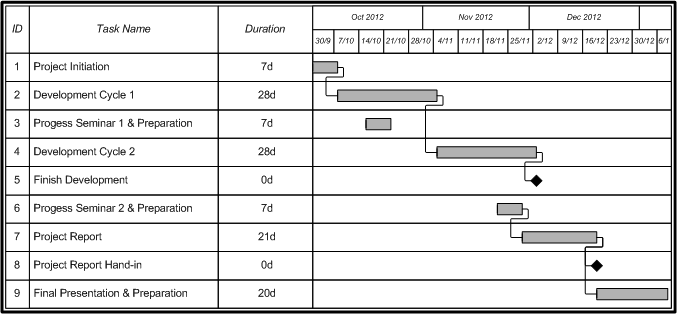
\includegraphics[width=0.8\textwidth]{img/l1plan.png}
\caption{Level 1 Plan}
\label{fig:l1plan-1}
\end{figure}


Once the group had established an initial breakdown of the tasks involved with the
project and a general idea of the approaches the group could take,
 a skills audit was held to discuss which team members were best
qualified for the various roles required by the project. The table below shows
a summary of the audit including the skills relevant to the approach taken.

\begin{center}
%\begin{table}
\begin{tabularx}{\linewidth}{|XXX|}
\hline
Group Member & Skill & Level of Expertise (1-5) \\ \hline
Thomas Grainger & Python & 5 \\
& Python Frameworks & 3 \\
& Distributed Systems & 4 \\ \hline
Weike Liao & Python & 3 \\
& Distributed Systems & 4 \\ \hline
Chris Orchard & Python & 4 \\
& Project Management & 3 \\
& Systems Integration & 5 \\ \hline
Nafiseh Vahabi & AI & 5 \\
& Python & 4 \\
\hline
\end{tabularx}
%\end{table}
\end{center}

%maybe more stuff about streams of work?
After some background research had been performed, the group decided to split
the development tasks into discrete components allowing members of the group to
work in the areas of most experience, using their specialist understanding of a
given area to research and develop in an autnomous fashion with progress and
code produced periodically reviewed by the other members of the group. The
individual streams of work should meet at the customer milestones to allow some
integration testing and to present some new working functionality to the
customer.

\subsection{Group-work Approach}
%TODO: elaborate to an appropriate extent
The development approach used for the project draws inspiration from agile
methods, with two
development iterations over the 10 week life of the project. Whilst ideally more
iterations would be made, allowing more customer involvement, the
structure and timescale of the project meant that this was not possible. If
there had been more available development time, the project would have defined
phases for the inception and elaboration of the project following a Unified
Process approach \cite{jacobson1999unified}, instead the inception and elaboration tasks are
interleaved into the first development iteration as shown on the Gantt charts. 

At the time of the skills audit, the group also investigated appropriate tooling
for the development to be carried out. The programming language chosen to implement the
solution in was python, as all of the group members had some experience
with the language, and it was also noted that python code was generally easier to
read than some of the other options available, making code review somewhat
easier. Another advantage of choosing python was the inclusive developer
community, allowing the group to contribute a bug fix back to one of
the tools used by the project, utilising some prior experience in python distributed
frameworks.
For version control, git was chosen as most of the group had previous experience
with the tool, and the group also chose to use GitHub to host the code
repository (in a private repository) removing some risks associated with the
possibility of ECS systems failure. GitHub gave the group an easy way to monitor
commits and view the diff made by any given commit, a feature that made the
process of reviewing committed code much quicker. GitHub also presents a
RESTful API that the group
found useful for developing metrics tools. This report is written in LaTeX,
mainly to ease the burden of version control and collaborative editing by using
multiple files, but also to enable metrics to be generated for report progress
during the write up.

%adjust to say less not-production-ready?
Choosing and enforcing an appropriate level of quality control for the code
developed was an important task throughout the project. The customer specified
that they would prefer a solution along the lines of a high-fidelity prototype,
as a way of achieving a maximal amount of useful work, with further testing to transition
to a production-ready system if the developed product proved to be useful
(outside of the scope of the project). This
is not to say that the code was not tested and reviewed throughout the project,
just that testing and review were not enforced as vigorously as might be
required for direct production use.

%example of use cases, use cases??!
At a very early stage of the project, the use of a distributed task framework as
a platform for the project was considered the preferred way to construct the
project, and this design decision was made for a variety of technical reasons
detailed in the technical approach section of this report. There are also some
benefits for managing the development effort from using such a framework. The
framework allows each component to be developed in relative isolation from the
other components, with low coupling between the different parts of the system.
This also served as a method for mitigating some of the risks associated with
individual components in the system either not working, or not being suitable
for a given use case when deployed by the customer.

During the development of the project, the group had to make two presentations
detailing the progress made up to that point, addressed to the supervisor,
customer, and a selection of peers. The Level 1 plan above shows the gaps left
for the preparation of each presentation. For each presentation, the group first
came up with an appropriate structure for the presentation, and then constructed
the relevant slides according to which parts of the work being presented each
member of the group was responsible for. An equivalent process will be used for
the end of project presentation.


\subsection{Risk Management}

As part of the project management task, possible risks associated with the
project were identified, and steps taken to mitigate them. The risks identified
by this process are listed in the table below. Throughout  the
project, precedence was given to tasks with outstanding risk, or risks that had
not been assessed, as a means of minimising the risk of the project not being
finished by the deadline.

\clearpage
\begin{landscape}
%\thispagestyle{empty}
%\makebox[\textwidth]{
\small
\setlength\LTleft{0pt}
\setlength\LTright{0pt}
\begin{longtable}{@{\extracolsep{\fill}}|p{5cm}p{1cm}p{2cm}p{6cm}p{2cm}p{2cm}l|}
    %\begin{tabularx}{1.5\textwidth}{|p{5cm}XXp{5cm}XXl|}
        \hline
        Risk & Impact (1-5) & Probability (1-5) & Mitigation & Risk Score (1-25) & Mitigated Risk Score & Status \\ \hline
        The delivered project does not meet the provided specification. & 5 & 2 & Ensure that progress is monitored throughout the project and any necessary change in specification is discussed with the customer. & 10 & 8 & Not Impacted \\
        \hline 
        The delivered project does not meet customer expectations & 5 & 2 & Ensure customer is aware of the status of the project and likely outcome throughout the course of the project lifecycle & 10 & 4 & Mitigated \\ 
        \hline
        A tool or library chosen for the development of the project does not meet its requirements. & 4 & 3 & Select tools and libraries that group members are familiar with, and preferably those which can be patched by group members where possible. & 12 & 6 & Mitigated \\ 
        \hline
        Integration takes much longer than planned due to conflicting styles of coding in software components developed by different group members & 3 & 4 & Discuss and enforce a single style of coding for all software, reviewing code as it is written. & 12 & 3 & Mitigated \\
        \hline
        The code contributed by a team member does not perform as expected or is not completed to the necessary quality & 4 & 2 & Review all code committed to the source repository, use pair coding if possible. & 8 & 4 & Not Impacted\\
        \hline
        A group member struggles with a task due to not having the necessary skills to perform the task & 4 & 2 & Use a skills audit to determine the confidence of the group members in various tasks, and allocate work accordingly. Monitor progress throughout the project and re-allocate work if necessesary & 8 & 4 & Mitigated \\
        \hline
        Interaction with the customer leads to a significant expansion of scope of the project, causing the project not to be delivered on time. & 5 & 2 & Be vigilant of any possible scope creep, and discuss the implementation time of any requested changes with the customer. & 10 & 6 & Not Impacted\\ 
        \hline
        Infrastructure hosting critical parts of the project such as the source code repository suffer from a critical failure, preventing access or causing loss of work. & 5 & 2 & Use a distributed version control system such as git for all code and written documentation, hosted on a large reputable code hosting service such as GitHub.  & 10 & 2 & Mitigated\\
        \hline
        A member of the team falls ill, preventing them from contributing significantly to a given part of the project. & 5 & 2 & Ensure a low "bus factor" is maintained, and that no single group member is given responsibility for a larger than necessary portion of critical tasks. & 10 & 8 & Not Impacted\\
        \hline
        The group is not given the necessary permissions from iSolutions and JANET to operate the project on university systems. & 4 & 3 & Communicate the intent and reasoning for the project at an early stage, ensure suitable preventative measures are implemented to prevent adverse effects from the malware scanning component of the project. If possible, keep a group member's personal computer as a contingency. & 12 & 6 & Mitigated\\
        \hline
        ECS are not able to provide the group with the resources necessary to run the project. & 4 & 1 & Request sufficient resources at an early stage, track the resource usage of the project during development and attempt to keep resources used during scanning to the minimum necessary & 4 & 2 & Not Impacted\\
        \hline
    %\end{tabularx}
\end{longtable}
%}
\end{landscape}
%Risk approach???

\subsection{Stakeholder Management}

%TODO:JANET explanation
%TODO:call isolutions isolutions?
%are supervisor/second supervisor stakeholders?
Although interaction with the customer has been detailed previously, there are
also some other stakeholders of note, specifically in relation to the use of the
University of Southampton's infrastructure and JANET's network link to
potentially download (and try to execute in some cases) large volumes of
malware. A solution was found to the technical challenge of how to restrict
possible malicious activity caused by malware being analysed by the system, as
discussed in the technical approach. Once the preventative technical measures
had been discussed with members of ECS systems staff and judged adequate, both
JANET and the University computing service were contacted to inform them of the
intended activity, and to invite comment. A conversation ensued with the
technical staff of the University infrastructure team, who not only felt that
the measures being taken were adequate but was a model solution of how such work
should be carried out in the future. All of the contact detailed above took
place via the groups single point of contact for the stakeholders. Although
having a single person responsible for all stakeholder contact is not risk
averse, this is offset by the advantage of the stakeholders only having to deal
with a single person, not having to link together several email addresses or
identities, and mitigating the risk of the conflicting messages being sent to a
stakeholder from different group members.


%justified design
\section{Architectural Design}
\subsection{Design}
The project can be split into four phases of operation, Trend Source Analysis, URL Discovery, Malware Detection and Result Storage in a persistent database.

This section of the report describes the design of a framework that connects those phases of operation together in a distributed manner.

\subsubsection{Components}
\paragraph{Trend Analysis}
Each trend analysis phase should be able to query some external services and determine a set of keywords. These keywords can then be returned, to be expanded to URLs by the URL Discovery phase.

\paragraph{URL Discovery}
The URL discovery phase is called with a keyword or trending topic from the Trend Analysis phase and should be able to determine URLs related to that keyword. This phase is designed to emulate a user searching for pages given a keyword.

\paragraph{Malware Detection}
The malware detection phase will accept a single URL, and optionally the keyword that resulted in the discovery of that URL, returning a confidence level that the URL resolved to malware.  This confidence can be combined with a static overall confidence level for the particular malware scanning method used.

\paragraph{}
Originally the system was designed with multiple different types of malicious content in mind and so each malware scanner was required to return a ``type'' of malware as well as a confidence level. After a meeting with the customer, however, in which it was clarified that only drive by download malicious content should be focused on the only valid ``type'' is ``generic''.

\paragraph{Result Storage}
To store the results of the system the response from a malware scanner must be associated with: the URL that called the malware scanner, the keyword or trending topic that was used to discover the URL, the trend source that the topic applied to and the particular components used in forming the result.

\subsubsection{A Distributed System}
To be able to operate quickly the system can be organized into a parallel architecture. This is due to the independent nature of many components of the system: Trend Source Analysis, URL Discovery and Malware Detection.

\paragraph{}
Each trend source is not dependent on on any other trend source, however the search engine tasks cannot be dispatched without a keyword from the Trend Analysis phase to be able to operate.

\paragraph{}
The process of scanning and determining if a URL has at one point returned a malicious page or not is entirely independent of both any other URL or any other particular method of scanning.

\paragraph{}
As such multiple sources can be queried for trends and those trends can then be used to browse for URLs using search engines, while multiple malware scanners are able to operate on multiple discovered URLs at the same time.

\subsection{Implementation}
This section describes how to use a set of workers to determine trending topics and sites relating to those topics

\subsubsection{Tools}
\paragraph{Celery}
Celery is a ``Distributed Task Queue'' that allows standard Python functions to be converted into Tasks that can operate asynchronously and in parallel on a large cluster of worker machines.  These Tasks can be dispatched in real-time or can be scheduled to take place at a particular time in the future, or at a predictable time intervals.  This scheduling feature is particularly useful for this project because it is required to schedule a complete flow through all phases of operation each day.

% TODO: Make sense
\paragraph{}
Celery Tasks can either be executed: while the calling thread waits until the Task has finished,  asynchronously by the calling thread that then ignores the result (useful in cases such as adding information to a database) or the calling thread can add a new Subtask to be called with the result of the previous as its argument.

\subparagraph{}
The Celery Subtask is a serialize-able version of a Task and describes the arguments, and the function name so that it can be sent to another worker to be called later.  The Subtask can also be used in a similar way to partial functions, so that more arguments can be added to a Subtask in different steps before it is finally called.  This is useful because it means that a range of Subtasks can be created that all share a predefined value: a particular Trend Source and then can be added as an asynchronous callback to be later given a specific argument: the particular Trending Topic from that Trend Source.

\paragraph{Threading Models}
Celery supports multiple threading models including multiprocessing and Eventlet.
\subparagraph{multiprocessing}
Part of the Python Standard Library, multiprocessing, is a threading model that spawns separate processes in which to consume execution units.  This means that each thread is very resource intensive because it is a full process and requires all of the code and a complete instance of the Python environment.

\subparagraph{Eventlet}
Eventlet is a wrapper around either epoll or libevent both of which provide a ``mechanism to execute a callback function when a specific event occurs on a file descriptor'' such as a notification on receiving data in a TCP socket. 

\subparagraph{}
For programs to be able to take advantage of Eventlet's support for fast non-blocking IO operations they must be written specifically with Eventlet in mind by using ``green'' threads, or ``coroutines''.  Usefully as part of the Eventlet library versions of Python libraries that can be used to make HTTP requests have been created that are built to work co-operatively in an Eventlet environment: \emph{urllib} and \emph{urllib2}. The \emph{requests} library which uses \emph{urlib3} has support for Eventlet built in already.

\subparagraph{}
Potentially thousands of ``green'' threads can be spawned with minimal resource usage, but any blocking operation causes the entire pool to block also. This is more useful than the multiprocessing threading model for most phases of the system as the majority of them spend most of their execution time downloading data from the Internet.

\paragraph{Message Brokers}
To be able to communicate to multiple workers operating on multiple, disparate and networked machines Celery requires a message broker and a result back end to make results of Tasks available to other Tasks.  The recommended message broker is RabbitMQ.

\subparagraph{RabbitMQ}
Although being one of many possible message brokers, RabbitMQ was chosen as the message broker not just because it is the system recommended by Celery.

\subparagraph{}
Celery supports a range of message broker systems, two message queue systems: RabbitMQ, and Beanstalk, three NoSQL databases: Redis, MongoDB and CouchDB and any SQL database supported by SQLAlchamey or the Django ORM.

\subparagraph{}
While some of the database systems support publish and subscribe on records none of them are capable of managing multiple queues of messages on widely distributed machines.  The SQL databases are to be particularly avoided and only used for test or because no other system is available. This is known as the ``Database as Queue Anti-pattern''\cite{database-as-mq}.  Using a database as a queue is an anti-pattern because the only way to get notified of messages is to repeatedly poll the database and also because a database is difficult to share among multiple client machines while remaining synchronized.

\subparagraph{}
The only remaining systems after the others have been eliminated are Beanstalk and RabbitMQ, both message queue systems. RabbitMQ was chosen over Beanstalk because it is easier to distribute the broker itself over a group of networked machines when using Rabbit MQ using the Shovel plugin.

\paragraph{Django Object-relational Mapper}
An Object-relational Mapper or ORM creates an object orientated interface to relational database systems.  This means that rows in a database can be created and interacted with in a way similar to native Python objects.

\paragraph{}
Popular libraries in Python include SQLAlchemy and the Django Object-relational Mapper. Because the system should be able to interface with a Django web interface to display results the Django ORM is an obvious choice.

\subsubsection{Parallel Crawling and Scanning Framework}
Each Task is implemented as a Celery Task in its own module, \verb`source`, \verb`search` and \verb`scan` depending on the phase of that Task: Trend Source Analysis, URL Discovery and Malware Detection respectively. Each phase module exposes the Task entry points with a list of functions.

\subsubsection{Controlling the Phases and Storing the Results}
The general approach to controlling the system is to allow data to flow from the source tasks via the the search tasks to discover URLs to be dispatched to scan tasks. Ensuring that each result from a \emph{Trend Analysis} task results in a new \emph{URL Discovery} task.  Each result from the \emph{URL Discovery} tasks should results in a new \emph{Malware Detection} task.  Finally each result from the \emph{Malware Detection} tasks are stored and related to the relevant Keyword and URL.

\paragraph{}
However two different technical approaches were applied to control the flow of the system:

\paragraph{}
One in which a single task, the scheduled task, controlled the entire process.  Ensuring that each phase completed and waited before starting the next, gradually building a Python data-structure out of dictionaries and lists until finally returning it.  This structure can then be validated and finally written to the database in one go.

\paragraph{}
The second approach used, making use of a Celery a Task for each phase of operation.  In which each \emph{phase controlling task}: inserts the results from the previous phase into the database, manages the dispatch of the different types of Task of that relevant phase, and passes on those database objects as a parameter to a partial task of the next phase to be used as a callback.  This effectively results in the \emph{phase controlling tasks} passing Django ORM database objects through the system, finally writing each result into the database at the end of the task.

\paragraph{}
Tasks which call the database using the Django ORM block and will therefore block the operation of all Eventlet tasks on the worker because the Django ORM was not written with green threads in mind.  Therefore the multiprocessing threading model is required, so all of the \emph{phase controlling tasks} must be routed to a worker that uses multiprocessing.

\paragraph{}
The second approach was chosen as the final approach and is justified in the Testing section.

\subsection{Testing}
\subsubsection{Placeholder Malware Scanning Task}
A simple Twitter source Task and Dogpile search Task could be developed very early on in the project and it is also possible to reduce the workload of the system by changing the Dogpile search engine to only query for the first page of results, as such significantly less URLs will be processed.

\paragraph{}
Malware detection Tasks, however, require significantly more in depth technical work before they become operational and would not be expected to be complete before nearer the end of the project. Therefore before being able to demonstrate and test the distributed framework a placeholder malware scanning task was produced. This task downloaded the contents of the page referenced by the given URL using \emph{requests}, loaded the document into an \emph{lxml.html} object and returned the contents of the \verb`<title>` element of the document or ``Failed'' if there was no title, or an \emph{Exception} was thrown.

\paragraph{}
Despite this process being unable to give a useful result, due to the title of the returned document having little to no bearing on whether or not that page is malicious, it served to both allow the system as a whole to operate and act as a template for other group members when developing parts of their code.

\subsubsection{Creating A Demonstration}
As part of the first presentation it was decided that a demo should be used to show how the project had developed.  In this demo the first approach was used to generate a JSON file representing the data that would be inserted into the database.  While this approach is acceptable for a small number of tasks the requirement to block operation when waiting for each phase to complete is unacceptable in the final system, so the second callback oriented, asynchronous approach was used.

\subsubsection{Considerations For ECS systems}
Thanks to Celery the system can scale to very large clusters of machines, however the implementation used to test the system was the minimum required to demonstrate the ability to work over some number of machines: Two Virtual Machines, one controlling node hosting a RabbitMQ server and another purely worker node.
\subsection{Testing}
The program's individual functions were tested separately. The sequence of 
testing was as following:
\begin{enumerate}
\item Downloading and parsing of HTML.
\item Extraction of links and make them absolute.
This was tested by printing all links as absolute from a given HTML and checking 
manually.
\item Removal of duplicate links and those links to other domains.
\item Downloading of an arbitrary URL.
This function was tested by downloading testing websites such as
\verb`http://www.thinkbroadband.com/download/`
The tests with various file 
sizes passed without errors and those links that exceeded the size or time limits were 
ignored. 
\item Clamd scan of the downloaded contents. 
\end{enumerate}
\paragraph{}
After that the whole program was tested with benign websites which provide 
testing for various viruses. These files used for testing were not real viruses however anti-virus packages recognize these signatures 
as part of their test suite. 
One of the websites used was Eicar\cite{eicar}. This website provides a small test 
virus in three compressed levels: plain text, zipped and double-zipped, with 
download links in the same page. The results obtained after 
crawling the web page are presented below:
\begin{verbatim}
[('http://www.rexswain.com/eicar.com', 
{'stream': ('FOUND', 'Eicar-Test-Signature')}), 
('http://www.rexswain.com/eicar.zip', 
{'stream': ('FOUND', 'Eicar-Test-Signature')}), 
('http://www.rexswain.com/eicar2.zip', 
{'stream': ('FOUND', 'Eicar-Test-Signature')})]
\end{verbatim}
Consequently the unit testing of the ClamAV scanner was successful. 

\subsection{Evaluation}



\clearpage
\section{Classification}

\subsection{URL Classification}

Recent studies on malware detection appears to show the idea of applying classification algorithm has became more popular. The classifier applied tries to separate the malicious data from the clean data. Therefore, in all cases a binary classifier has been used. One of the requirements when designing a classifier for the detection system is to have a dataset in advance. The dataset is used as an input for the classifier. Therefore, having a classifier saves resources and makes the system more efficient and robust.Research has been performed to design a system to detect a malicious dynamic HTML code with the aid of a variant classification algorithm. The researchers compared the performance of their system with some anti virus software. The result of their comparison indicates the tolerance of anti virus software is between 40\% and 80\%. This observation shows the lack of intelligent malware detection system that detects any type of attack. Most anti virus software used signature-based technique for malware detection\cite{Macilious-web}  
 The following section describes the details of the classification algorithm employed for this project. 
\subsubsection{Design}
The classification algorithm is made up of two main units, the URLs database and the classifier unit. Figure \ref{fig:clas-1} demonstrates the architecture of the classification module.

\begin{figure}[htb]
\centering
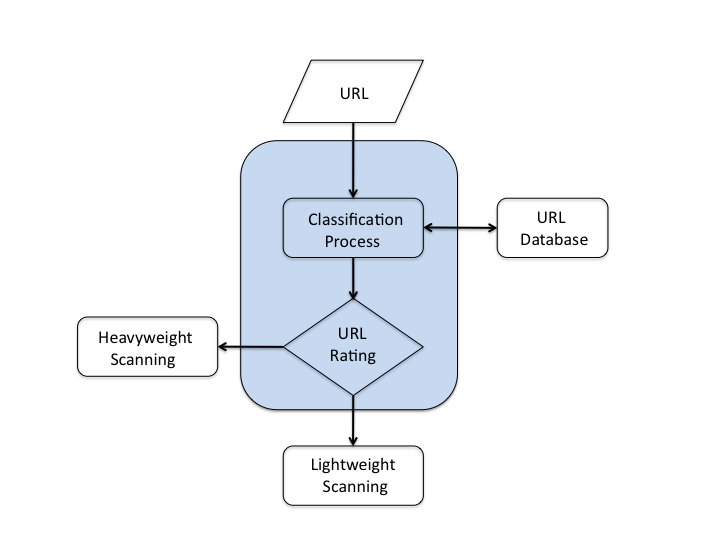
\includegraphics[width=0.8\textwidth]{img/classification(diag).png}
\caption{Classification module architecture}
\label{fig:clas-1}
\end{figure}

% inserted the image of the flowchart for the classification algorithm


\paragraph{} 
The URLs database contains a list of URLs that specifies whether that URL is malicious or not. The URLs database will receive feeds from five different sources, being five different malware detection systems.The second component of the classification algorithm is the classifier unit. A new URL first enters the classifier unit and the classifier checks the structure of the new URL against the structure of URLs listed in the database. Based on the classifier algorithm decision, there will be three outcomes for the maliciousness of the new URL. If the new URL already exists in the database the classifier will immediately confirm whether or not the URL is malicious and hence there is no need to perform more scanning on that URL. However, if the URL does not exist in the database and the classifier returns a poor confidence rate then the new URL needs to be subjected to the heavyweight scanning process. Otherwise, the URL will follow the lightweight scanning process. Section 2 explains the implementation of the classification algorithms in more detail



\subsection{Implementation}

\subsubsection{URL Database}

An important part of the classification algorithm is the dataset used for the purpose of the clustering. The dataset in this project contains examples of both malicious and benign URLs. 

\paragraph{} 
The results from the five malware scanners along with the associated confidence rate is saved to the classification database. Therefore, after running the detection system, the database is updated and the new URLs are added to the database. For the purpose of pattern matching, the system developed includes the capability of converting the contents of the database into the Python dictionary.

\subsubsection{Classification Unit}
 
The classification unit is where the data clustering is performed. Initially, the plan was to employ the machine learning methods in the classification algorithm. The most popular machine learning methods for clustering are; Naïve Base, Support Vector Machine (SVM) and Decision Tree. Employing the machine learning methods requires a predefined dataset to build the training and learning dataset. Therefore, any unknown URL can be identified based on the learning data. According to the observation of the deSEO research and IMDS project, the results will be reliable and promising\cite{deseo}.
However, despite the initial plan and advantage of using machine learning methods for the classification, it was not possible to apply such methods in this project for the following reasons:
\begin{enumerate} 
\item The project is time limited 
\item The result of malware scanner modules will not be available until the end of the project.
\end{enumerate}
Therefore, an alternative approach was adopted for the classification unit. This relies on pattern matching between two URLs, one being the new URL and the other the database URLs. For pattern matching, each URL is deemed to be a string, so an algorithm is required to perform the matching between the two strings. A few string measurement algorithms were attempted with the most suitable being selected. A brief description of the attempted algorithms are provided below;

\paragraph{Fuzzy String Searching}
			
This is a technique used to search for the closest match for a given string. It is also called Approximate String matching. As its definition suggests, this technique does not produce an exact match for a given sequence. Furthermore, its implementation is complex and the algorithm is quite slow \cite{String-match}.

\paragraph{Sequence mining}

Sequence mining is a popular algorithm used in data mining. Data mining is a process to find a pattern in a dataset. This algorithm tries to find similar patterns between two sequences and is used in Bioinformatics and for predicting DNA sequences. Sequence mining algorithm is remarkably efficient, and this attribute makes the algorithm suitable for implementing in other applications. However, the algorithm is used for sequences that have a restricted number of alphabet characters. Therefore, given the variation of URLs in the dataset, this algorithm is not appropriate for this project\cite{Sequence-mining}.  

\paragraph{Jaro–Winkler distance}

The Jaro-Winkler distance algorithm is popular in computer science and is also applied in statistics. This algorithm aims to find similarities between two strings by assigning a confidence rate ranging from zero to one to the result of the algorithm. If the result is zero, there is no similarity between two strings, whilst a result of one means there is an exact match for the two strings. This method gives an accurate result when comparing short strings such as a person’s name. However, for lengthy URLs, the application of this method produces a poor result. Therefore, this method is rejected for use in the implementation stage because the result would only be reliable for short URLs\cite{Jargo-winkle}. 

\paragraph{Levenshtien Distance}
	
Levenshtien distance is one of the strings metrics that measures the minimum number of edits required to convert one sequence to another. It is sometimes called edit distance. In this measurement the following edit operations are permitted; deletion and insertion. 
For example, the Levenshtien distance between ``http://www.bbc.co.uk/news/world/'' and ``http://www.bbc.co.uk/news/wales/'' involves four steps before the first URL is converted to the second, as shown below:
\begin{enumerate}
\item 
{\bf substitution of `a' for `o'}\\
\url{http://www.bbc.co.uk/news/world/} to \url{http://www.bbc.co.uk/news/warld/}
\item
{\bf deletion of `r' }\\
\url{http://www.bbc.co.uk/news/warld/} to \url{http://www.bbc.co.uk/news/wald/}
\item
{\bf Insertion of `e' after `l'}\\
\url{http://www.bbc.co.uk/news/wald/} to \url{http://www.bbc.co.uk/news/wale/}
\item
{\bf Insertion of `s' at the end}\\
\url{http://www.bbc.co.uk/news/wale/} to \url{http://www.bbc.co.uk/news/wales/}
\end{enumerate}

\paragraph{} 
According to the Levenshtien distance, it is not possible to transform the first URL to the second one with fewer than four edits. The main advantage of using this method is that two URLs do not need to have the same number of characters. Hence, a URL with any structure is acceptable as an input for the classification. However, adapting the Levenshtien distance for pattern matching can reduce the speed of the system.

\paragraph{} 
After analysing different methods for pattern matching and considering their advantages and drawbacks, the Levenshtien distance was selected and implemented in the classification.  Therefore, when a new URL enters the system, the classification unit searches the database to find a match to the new URL. There are three possibilities as a result of this matching. Firstly the new URL may already exist in the system; in which case a result is immediately returned with a one hundred percent confidence rate. The latter result determines whether the new URL is malicious or benign. The second possible outcome of the classification unit is that a result is returned with a poor confidence rate. In this case the new URL will be sent to the heavyweight scanning module to undertake further scanning. Thirdly, a pattern matching result showing a high confidence rate would follow the lightweight scanning process.
The advantage of incorporating a classification module within the malware detection system is increased efficiency. More importantly, the system is capable of identifying unknown URLs, which many commercial virus scanners are not able to detect. 

\clearpage
\section{Trend Analysis}
\subsection{Design}
Trend Analysis Tasks should be implemented to take advantage of multiple different sources of trending topics to be used as keywords for URL Discovery tasks.

\paragraph{}
Sources that the system will use include the Twitter Trending Topics API, RSS Feeds and trends from derived from the Sun JSON Feed.

\subsubsection{Twitter}
The Twitter API is available in multiple versions, 1 and 1.1. Currently 1 is deprecated and it is recommended that new applications build against 1.1.  The disadvantage of the 1.1 API is that it requires a ``User Context'' so all requests must be performed as an authenticated user.This requires both a Twitter User and Application OAuth token.

\paragraph{}
As part of the Twitter API access to global trending topics is made available at a JSON endpoint\footnote{\url{https://api.twitter.com/1.1/trends/place.json}}. This is possible to parse manually but a library should be chosen to handle the interaction and authentication instead.

\paragraph{}
Topics with a pound sign ``\#'' as the first character are Twitter ``hashtags'' and are usually camel cased. But these hashtags must be converted from camel cased to space delimited so that the topic can be used as a set of keywords. For example ``\#BrazilWantsOneDirection'' becomes ``Brazil Wants One Direction'' and ``\#XFactorPHFinale'' becomes ``X Factor PH Final''.

\paragraph{}
In the case of all capitals eg ``NIALLSAYHITOTURKEY'' an entirely lowercase keyword should be derived.

\subsubsection{RSS}
A set of RSS feeds should be collected and parsed, ``feedparser'' is likely to be useful for this.  Each item from a feed should be entered into a corpus, to calculate keywords from items in the corpus algorithms such as TFIDF should be used. The natural language library ``metanl'' is likely to be helpful. Note that each feed can be processed separately with one corpus per feed.

\subsubsection{The Sun JSON API}
The Sun provides a JSON API for the top 200 most commented on articles\footnote{\url{http://bootstrap.thesun.fyre.co/api/cust/ni/todays_hottest/200.json}}. In most cases the content of this JSON file can be treated in exactly the same way as an RSS feed however care should be taken to deal with the strange encoding of some of the returned headlines: \verb`Terry a â\u0080\u0098liarâu\u0080\u0099` should be \verb`Terry a "liar"`.

\subsubsection{Alternative Sources}
Examples include:
\begin{itemize}
    \item Link aggregation sites such as Reddit and Digg.
    \item Search engine common searches and trends such as Google, Bing and Yahoo trends services.
    \item Network logs such as the campus search trends. It should be noted that this data is very unlikely to be accessible by malware distribution networks and might allow us to see trends before they do.
\end{itemize}

%implementation
\subsection{Implementation}
The most popular Twitter library for Python is called Tweepy, which is also 
our choice. This library provides access to Twitter version 1.1 API, which 
requires OAuth authentication. Therefore we created a Twitter account 
dedicated for this program, which provides consumer key and access token in 
order to pass the authentication. \\
The program then retrieves global trending keywords from the Twitter's {\em 
trends/place} API. As previous described, in order to cope with keywords with 
hashtags, we implemented a hashtag handler, who's role is to remove the hash 
tag and convert the camel case word to sentence case. This is achieved by 
applying regular expression substitution: 
\begin{verbatim}
re.sub(r'((?<=[a-z])[A-Z]|(?<!\A)[A-Z](?=[a-z]))',r' \1',
camelCaseString)
\end{verbatim}
Before the conversion happens the keyword is also decoded into unicode. The 
reason is that Celery does not support Python 2 strings with non-ASCII characters
which may lead to 
crash when Celery is sending them to RabbitMQ. 
\paragraph{}
A list of famous news websites' RSS feed addresses are hard coded in the 
program, the website list includes BBC, NewYork Times, Guardian, The Washington 
Post and so on. The RSS parser downloads every feeds, parses them into list 
then extracts news titles in them. Characters require encodings other than 
UTF-8 are ignored. The downloading is achieved with requests and any network 
errors will be handled in order to prevent system crash. 
\paragraph{}
The top 200 commented articles from Sun JSON API are handled in a similar way 
as that of RSS feeds. Due to good compatibility between Python and JSON the 
extraction of article titles were completed without any difficulties. 
\paragraph{}
Twitter trends, RSS feeds and Sun JSON are implemented as three different 
functions which are going to be run as separate Celery tasks. All of them 
return a list of keywords or sentences to the main system. 

\clearpage
\section{URL Discovery}
\subsection{Design}
\subsubsection{URL Discovery}
URL Discovery tasks are designed to discover URLs to be dispatched to Malware Detection tasks.

\paragraph{}
Search engines are built specifically for this task, as such this Task is designed to query a search engine to determine a set of pages related to those URLs.

\subsection{Implementation}
\subsubsection{Dogpile}
Each of the popular search engine like the Google Search, Yahoo Search and Microsoft Bing search engines employ techniques to prevent the scraping of their results because of the commercial interest to keep those results proprietary so as to gain advertising revenue.

\paragraph{}
Instead meta-search engine Dogpile was used, Dogpile obtains results from Google and Yahoo and provides those same results in very simple to screen-scrape HTML:

\begin{verbatim}
map(
    lambda link: link.get('href'),
    lxml.html.fromstring(
        requests.get("http://www.dogpile.co.uk/search/web?q=foo").text
    ).cssselect(".webResult .resultDisplayUrl")
)
\end{verbatim}

\paragraph{}
However each of the links we want is wrapped in a ``ClickHandler'', this click handler is used so that the referrer header with the topics used in the search are not sent to the result page when it is followed by a user.

\url{http://cs.infospace.com/ClickHandler.ashx?du=http%3a%2f%2fwww.ietf.org%2frfc%2frfc3092.txt&ru=http%3a%2f%2fwww.ietf.org%2frfc%2frfc3092.txt&ld=20121006&ap=10&app=1&c=uk.dogpl&s=dogpileuk&coi=239138&cop=main-title&euip=XXX.XXX.XXX.XXX&npp=10&p=0&pp=0&pvaid=1351848139fc4226b6b6a0f6e0eed58b&ep=8&mid=9&hash=22AE450C7F5B9FA7C51FE2CEA7841093
}

\paragraph{}
As such the URLs in the page must be parsed using ``urlparse'' to retrieve the true, unwrapped URL available in the ``du'' or ``ru'' GET parameter\cite{rfc3092}.

%BEGIN INCLUDED TECH SECTIONS HERE
\clearpage
\section{Malware Lists}
\subsection{Design}
Malware list scanners are a type of Zero Interaction Malware Scanner. This means that these scanners do not interact in any way with the target server that is being investigated, specifically they do not download the page content. This is an advantage both because potentially less web requests have to be made and importantly the target server cannot detect this type of scan.

They use a collection of URLs or domain names that are pre-generated and made available by other systems such as WOT and Alexa.
\subsubsection{Services}

Alexa is a service that maintains a list of domains ranked by traffic. This traffic rank is determined ``by analyzing the Web usage of millions of Alexa Toolbar users and data obtained from other, diverse traffic data sources.''\cite{alexa-about}. This list is available as a zipped CSV that is updated daily\footnote{\url{http://s3.amazonaws.com/alexa-static/top-1m.csv.zip}}.

\paragraph{Alexa}
To use the Alexa service the data in the the CSV must be made available, locally, to all of the worker nodes. A web request should not be made more than once per day to the Alexa service as this is a waste of bandwidth. As such a distributed database, with the ability to designate a master and many slaves must be used.

\paragraph{The Web Of Trust}
WOT makes available a JSON API endpoint\footnote{\url{http://api.mywot.com/0.4/public_link_json}} for querying a database of domains associated with values of ``Trustworthiness'', ``Vendor reliability'', ``Privacy'' and ``Child Safety''. These values are crowd sourced: ``Based on ratings from millions of web users and trusted technical sources''\cite{wot-about}. Because the system is scanning exclusively for potential malware only the ``Trustworthiness'' value is taken into account.

\paragraph{}
The API endpoint has a single (non JSONP) parameter; ``hosts''. Instead of accepting multiple values for parameter as is usual in HTTP server implementations - to match select multiple fields the WOT API requires each value to be delimited with `/' and the entire collection of values to be terminated with a trailing `/'\footnote{\url{?hosts=example.COM/www.EXAMPLE.NET/.../}. as apposed to \url{?host=example.COM&host=www.EXAMPLE.NET}}.  This has the chief advantage of reducing the number of bytes sent in each request.

\paragraph{}
The usage limits of the API are as follows\cite{wot-about}:

\begin{itemize}
    \item The API must only be called once every 10 minutes.
    \item A request for the same domain must not be made in any 30 minute interval.
    \item The number of domains in the HTTP request must not exceed 100.
    \item The size of the URL of the HTTP request must not exceed 8KiB.
\end{itemize}

\paragraph{}
To prevent exceeding the usage limit, WOT tasks that access the database must be batched and results should be cached across the entire distributed system with a timeout of 30 minutes.

\nomenclature{CSV}{Comma Separated Values file}
\nomenclature{WOT}{Web of Trust}
\nomenclature{JSON}{JavaScript Object Notation}
\nomenclature{JSONP}{JSON with padding}

\subsection{Implementation}
\subsubsection{Tools}
\paragraph{Redis}
Both systems require a distributed storage component that can allow any worker to edit data in a centralized manner while also being able to access that data locally. The system chosen for this was Redis\cite{redis} because Redis is already being used as part of Celery, it supports a distributed mode of operation and transactions.

\paragraph{}
Redis allows us to designate a write master and many read slaves. This master should be placed in some location all the worker nodes can access, and can in fact be distributed across multiple machines.  In the \emph{Prototype Deployment} one node was arbitrarily chosen to be this master. All the workers also have a slave set to mirror off of the master Redis instance.

\subsubsection{Alexa Specifics}
The Alexa scanning system is split into two Celery Tasks, \emph{update\_alexa} a task to be run by a daily Celery Beat Periodic Task and \emph{alexa\_malware\_scan} a regular Celery Task to be called by the crawling system.

\paragraph{}
The daily task \emph{alexa\_top\_million} downloads the zipped CSV file of the top million domains, extracts the contained CSV file into memory. This CSV file is parsed row-wise using the CSV DictReader from the Python standard library. Finally, in a single transaction to the master Redis database, the previous value stored is deleted and a new Redis Hash value is created from the domain, rank mappings in the CSV. This transaction ensures that there is no point at which no data is stored in any of the slaves after the initial sync-up.

\subsubsection{WOT Specifics}
The Celery \verb`celery.contrib.batches` decorator is part of the celery API that allows multiple invocations of a single task to be buffered in a queue and executed at once with the entire collection of Celery Task request contexts made available at once. These request contexts are passed an as argument to the decorated function. This functionality is required because the WOT API allows multiple domains to be requested at once.

\paragraph{}
The WOT scanning system uses as a single Celery batches task \emph{wot\_malware\_scan}, backed by a regular Python function \emph{wot\_malware\_scan\_real}.

\paragraph{}
The batching task is configured to be run once 100 single tasks have been buffered or when 10 seconds have elapsed, this then passes an iterable collection of URLs to \emph{wot\_malware\_scan\_real}. \emph{wot\_malware\_scan\_real} returns an iterable of responses, in the same order as the URLs were requested. The batching task \emph{wot\_malware\_scan} then marks each single task request context as done, with the corresponding return value from \emph{wot\_malware\_scan\_real}\cite{celery-batches}.

\paragraph{}
The Celery \verb`celery.contrib.batches` task documentation did not describe how to return any results, as such this functionality had to be researched from some of the internal parts of the Celery library.  This research was written up and submitted to be included in the Celery documentation as a GitHub GitHub Pull Request and then later accepted\cite{celery-batches-docfix}.

\paragraph{Redis Cache Abstraction}
The Redis cache system is used to prevent the workers requesting the same data from the WOT API too often.  This was implemented using a caching function that can be used elsewhere in the project, abstracting away the caching layer.  The \emph{redis\_cache} function takes a \verb`key_prefix` to prevent collisions, a \verb`prepare` and \verb`request` function, and finally the set of \verb`items` that need to be requested.

\begin{enumerate}
    \item The \verb`prepare` function is used to process each item into the required part, for example parsing the domain out of a URL.

    \item The unique prepared items are requested from the local slave Redis database, and added to the total response. Any response from Redis where the result is False is a cache miss. The \verb`request` function is then applied to the collection of cache misses, updating the total response.

    \item Finally each \verb`item` discovered in the request phase is added to the remote Redis write master and the total response is returned.
\end{enumerate}

\paragraph{Usage of the Redis Cache Abstraction}
The \emph{wot\_malware\_scan\_real} invokes the Redis abstraction function with the following arguments:
\begin{itemize}
    \item \verb`key_prefix` ``malucrawl:web\_api:wot:{item}''.
    \item \verb`prepare` function that takes a URL and returns the domain part.
    \item \verb`request` function that, to meet the further requirements of the API guidelines, splits the domains into buckets limited to 8KiB and dispatches them as separate HTTP requests.
\end{itemize}

\subsection{Testing}
\subsubsection{Alexa}
The Alexa malware scanning system is very quick to test: there are no necessary buffer delays or complex caching systems. Each individual Task simply results in a single lookup in a local Redis instance, and there is no change from debug operation to full system operation.

\subsubsection{WOT}
\paragraph{Celery Batch Processing with Eventlet}
When the WOT Batch process task was executed for the first time using the Eventlet threading model the Celery debug log very quickly filled up with exceptions from the Eventlet and Celery libraries:

\begin{verbatim}
Traceback (most recent call last):
    File "/.../eventlet/greenpool.py", line 80, in _spawn_n_impl
        func(*args, **kwargs)
    File "/.../celery/concurrency/eventlet.py", line 50, in apply_target
        pid=getpid())
    File "/.../celery/concurrency/base.py", line 27, in apply_target
        callback(target(*args, **kwargs))
    TypeError: 'NoneType' object is not callable
\end{verbatim}

While these exceptions did not occur under the multiprocessing threading model, hinting that the problem might not be with the system code but in fact part of the Celery library itself.

The issue was determined to be part of the Batches API in which the Eventlet Green Thread Pool task was called with a NoneType callback, instead of a do nothing noop function.  This defect did not affect multiprocessing threads because a multiprocessing thread pool checks for a NoneType callback.

\verb`callback=acks_late[True] and on_return or None` became

\verb`callback=acks_late[True] and on_return or noop`

Where noop is a no-operation function and part of the standard ``utils'' available in the Celery library.

\paragraph{}
This change was delivered to the upstream community as a GitHub Pull Request and then later accepted\cite{celery-batches-fix}.

\paragraph{Debug Mode}
The Web Of Trust testing system when using a ten second delay before the Batches Task buffer is forcibly executed without waiting for 100 Tasks would be very slow thus making it difficult to make a change and verify if that change was correct. As such to prevent a stilted work-flow the delay is set to 0.1 seconds while the system is in debug mode (Controlled by a flag set in the Django settings file).  Meaning that the buffer is effectively emptied as soon as a single Task is requested.
\paragraph{Redis Caching Layer}
As part of the full system test, it was determined that Web Of Trust malware analyzer was returning results unrelated to the URLs it was being called with.

\paragraph{}
The offending line was tracked down to:

\verb`return [total_response[item] for items in item]` which should have been

\verb`return [total_response[item] for item in items]`

Where \verb`item` is the last \verb`item` left in scope after one of the previous python \verb`for` loops, that requested each item from or inserted each item into the cache.

\paragraph{}
This typo caused the data returned from the caching layer to only be relevant to a single item, meaning the bug is undetectable when only a single task has been buffered. Hence why it was only discovered after a complete integration test with the rest of the system.

% * into/malware type
% * APIs used
%     * WOT
%     * Alexa
% * Alexa
%     * celery beat ZIP download
% * WOT
%     * API requirements
%     * batch process, return items
%     * URL < 8Kio, <100
\subsection{Testing}
The program's individual functions were tested separately. The sequence of 
testing was as following:
\begin{enumerate}
\item Downloading and parsing of HTML.
\item Extraction of links and make them absolute.
This was tested by printing all links as absolute from a given HTML and checking 
manually.
\item Removal of duplicate links and those links to other domains.
\item Downloading of an arbitrary URL.
This function was tested by downloading testing websites such as
\verb`http://www.thinkbroadband.com/download/`
The tests with various file 
sizes passed without errors and those links that exceeded the size or time limits were 
ignored. 
\item Clamd scan of the downloaded contents. 
\end{enumerate}
\paragraph{}
After that the whole program was tested with benign websites which provide 
testing for various viruses. These files used for testing were not real viruses however anti-virus packages recognize these signatures 
as part of their test suite. 
One of the websites used was Eicar\cite{eicar}. This website provides a small test 
virus in three compressed levels: plain text, zipped and double-zipped, with 
download links in the same page. The results obtained after 
crawling the web page are presented below:
\begin{verbatim}
[('http://www.rexswain.com/eicar.com', 
{'stream': ('FOUND', 'Eicar-Test-Signature')}), 
('http://www.rexswain.com/eicar.zip', 
{'stream': ('FOUND', 'Eicar-Test-Signature')}), 
('http://www.rexswain.com/eicar2.zip', 
{'stream': ('FOUND', 'Eicar-Test-Signature')})]
\end{verbatim}
Consequently the unit testing of the ClamAV scanner was successful. 

\subsection{Evaluation}



\clearpage
\section{Capture-HPC}
\subsection{Design}

As one of the selection of high-interaction malware scanning
methods available for use in the malucrawl framework,
Capture-HPC\cite{capture-hpc} is a way of
realistically emulating a user browsing to a given URL in a real web browser.
Capture-HPC is designed as a client honeypot, where in contrast to the usual and
more common form of passive honeypots that simply wait for incoming attacks,
goes out and requests content from the Internet and attempts to detect any
malicious actions performed by the content. Capture-HPC was developed at Victoria
University in Wellington NZ and is maintained be the HoneyNet project\cite{honeynet}.

\subsubsection{Capture-HPC in Detail}

Capture-HPC uses virtualisation to simulate user browsing, using a web browser
running in a monitored and externally controlled Virtual Machine. There are two
distinct pieces of software used to do this, a client to run the web browser on
the virtual machine and monitor for malicious activity, and a server to
orchestrate URL scanning between however many clients are being used and to
reset client VMs when malicious activity is detected. The client and server
components communicate over a network connection.
\paragraph{The Client}
The Capture-HPC client is a C++ program that runs on Windows XP, Vista, or 7.
Its role is to automatically download content from the internet and to monitor
the VM for any
suspicious activity, reporting the outcome rendering URLs to the server. The
client is capable of driving a number of applications using URLS, from web
browsers such as Microsoft Internet Explorer and Mozilla Firefox, to downloading and opening
Microsoft Word documents and Adobe PDFs. For the purposes of the project, the
use of Internet Explorer is prioritised as a starting point for malware scanning
that can be easily extended to cover the other applications. To detect any
malicious activity that may be caused by visiting a website, or opening a
downloaded file, a collection of kernel drivers are used. The kernel drivers
watch filesystem, network and process activity at a low level inside the
operating system, ensuring that
unusual activity can be detected despite attempts from any malware to conceal
its actions. This isn't a technique that works in general on a PC where the user
may be performing any number of other actions whilst using the machine, but
works well in the controlled environment provided by the virtual machine. To
stop the small number of standard processes and filesystem changes made during
normal operation of the operating system and client applications triggering the
malware detection, Capture-HPC uses a set of "exclusion lists" that specify
actions for each monitoring tool that should be considered as safe. It is also
possible to specify precisely which actions should cause the monitoring tool to
report suspected malicious activity.
\paragraph{The Server}
The Capture-HPC server program that controls the clients is a Java program that
will run on most platforms (platform compatibility is limited by the VM revert
script detailed below). The role of the server is to communicate the exclusion
lists and URLs to be tested to the clients, and then collect the results of the
analysis. The server also uses an external script to reset the virtual machine
if malicious activity is detected by the client. The server also resets the
client if it does not respond to keepalive packets, so the client does not get
stuck on a URL that errors or a very large file such as a DVD. There exists two
options for supplying URLs to the
Capture-HPC server, using a plaintext input file with one URL on each line (the
line can also contain options controlling which client application is used to
open the URL) or a MySQL database with a schema provided with the application.
The server stores the results in text files labelled for safe URLs, URLs that
cause an error, dangerous URLS and the current
progress by default, with additional detail for suspicious URLs stored in a file
with the name of the suspicious URL (URL encoded). This is not ideal for use within
the project, but fortunately Capture-HPC will store all results in the
relational database if one is configured. URLs can be inserted into the
database, and when the server is run, the URLs are annotated with the results of
the scanning, with additional detail stored in other tables.
The use of a MySQL table for a queue
could be considered an anti-pattern as discussed in \cite{anti-queue}, but is the best of
the options available for providing Capture-HPC with data, and retrieving the
results, presenting an easiliy accessible interface for framework components to
integrate with wither locally or remotely. Unfortunately the Capture-HPC server
also has to be restarted to
consume new URLs from the database, with any finished URLs that are left in the
database processed again. The Capture-HPC server is configured using an XML
configuration file.
\paragraph{VM Integration}
The version of Capture-HPC to be used in the project supports VMware as its
virtualisation platform, and the ECS VM infrastructure also runs on VMware
products. Most VMWare products offer an API for programmatically interacting
with the Virtual Machines being hosted, known as VIX, and Capture-HPC uses this
API to reset VMs that detect any suspicous activity. The API however only has
bindings in perl and C,
so a bridging program written in C is supplied with Capture-HPC and must be
compiled independently of the server. Each virtual machine being used as a
Capture-HPC client needs to have the client software installed, and then a
snapshot taken. A VM Snapshot is a method of backing up the VM in manner that
preserves all information about the state of the VM, including the memory,
meaning that the state of the machine can quickly be restored to its original
after a malware detection. The bridging utility simply reverts the VM to the
first snapshot it can find, and then re-starts the Capture-HPC client. The
separation of the VM API component from the rest of the server proved to be
usefil in the project, as some modifications needed to be made to how VMs are
reverted, as detailed below.

\subsubsection{How Capture-HPC is used in the project}

Capture-HPC is the most accurate simulation of user browsing used by the project
as a malware scanner, and has a very low URL throughput thanks to each URL
needing to be rendered in a web browser. The throughput is further reduced 
the need to revert the VM every time malicious activity is detected. Therefore
it is necessary to limit the number of URLs that Capture-HPC is required to
process. As discussed previously, limiting of the URLs processed by the
high-interaciton malware scanners 
is done by a classification system, and only URLS that are strongly suspected to
harbour malware are submitted for scanning. In addition to the confidence factor
that each malware analyser in the framework must return, Capture-HPC is also
capable of returning a description of the actions taken by a malicious page, and
these details are returned to the framework for optional in-depth analysis. It
is also possible to calculate the ideal confidence value for a given classifier
and set of malware analysers working alongside Capture-HPC so that an optimal
set of URLs provided for time versus detection rate.

\subsubsection{Security Considerations}

As Capture-HPC renders web pages, there is a significant risk that any malicious
content will take over the client VM and try to exploit any other computers
connected to the VM or abuse resources in other ways such as sending spam.
To mitigate this threat, a set of preventative measures are taken. 
Figure \ref{fig:sec-1} shows the architectures used for the implementation of the security
considerations.

\begin{figure}[htb]
\centering
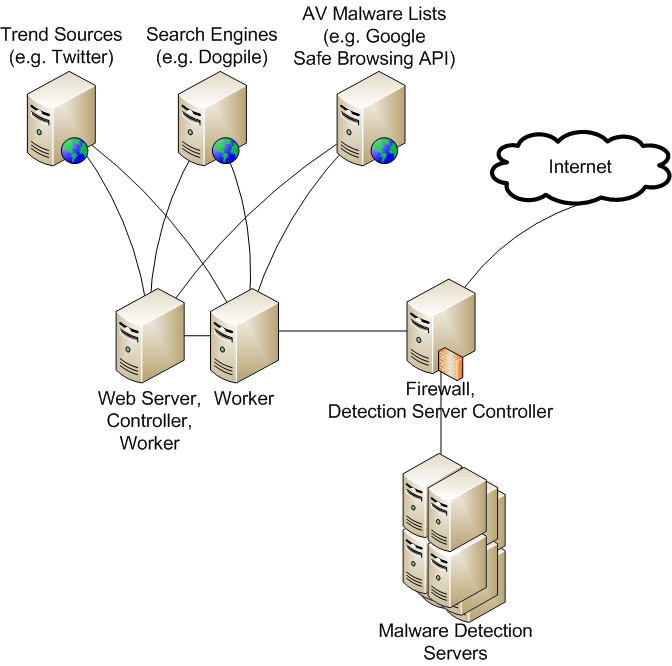
\includegraphics[width=0.8\textwidth]{img/physical-arch-pres.png}
\caption{Secure Architecture}
\label{fig:sec-1}
\end{figure}

To secure the virtual machine(s) running the Capture-HPC client, a Linux
firewall is placed between the VMs and the network, with the client VMs only
able to communicate with the outside network via the firewall. The firewall
blocks all ports by default, only proxying a small selection of ports and
forwarding no ports. To allow the Capture-HPC client to resolve URLs to IP
addressed, DNS
queries are proxied through the firewall, with all requests logged. All HTTP and
HTTPS requests are also proxied and logged using a weekly/monthly rolling log
so that any suspicious
activity can be investigated. A self-signed SSL certificate will be installed on
the client VMs so that HTTPS connections still appear valid despite interception.
A small selection of ports will also be open into and out of the firewall to
allow control of Capture-HPC and reporting of results, and to allow the
Capture-HPC server to communicate with the Capture-HPC clients.

\subsection{Implementation}

\subsubsection{Deployment of Secure Architecture In ECS}

%TODO: compiling client was difficult, but can port image to other platforms,
%re-use capture binary

When deploying Capture-HPC in ECS to form part of our prototype deployment of
the framework, a small group of VMs were used to host the security architecture
discussed above. The gateway VM used Red Hat Enterprise Linux 6 for its
stability and security,
with iptables used to provide a firewall. Squid was used as a HTTP and HTTPS proxy, compiled with
support for dynamically generating certificates for HTTPS websites. To reduce
the amount of effort needed to manually configure the firewall to allow/disallow
different types of traffic during
development of the system, a small tool was written to allow a number of
iptables "profiles" to be created, and then changed using a small shell script. Profiles were written for
development mode with little to no firewall restrictions but with NAT and
forwarding enabled, maintenance mode with restricted ports but forwarding with
NAT instead of proxying, and full mode with proxying and the minimum number of
open ports. The Capture-HPC Server program was also compiled and run from this machine.

The Capture-HPC client was compiled on a Windows XP development VM, and then
deployed to a clean install of Windows XP. Due to the complexity of compiling
the binaries, the installer generated in the build process is included with the
accompanying data package, but would unfortunately still need to be rebuilt for
use on versions of Windows other than XP. It is possible to run the
Capture-HPC client on a Windows Vista or Window 7 install, but was not tested in
the prototype deployment due to time constraints. The Windows XP install used
for the client had no anti-virus or firewall configured, with Internet Explorer
6 installed to present an easy target for malicious sites.

\subsubsection{ECS Specific Customisations}

The specific network architecture meant that some customisations had to be made
to the standard deployment, and to further reduce risk of malware escaping from
behind the firewall. The ECS VM infrastructure uses VMware vSphere to manage its
ESXi VM servers, and the Capture-HPC server must connect to the vSphere
administration console to revert the VMs when malicious activity is detected.
The VM administration API requires authentication, which uses ECS domain
credentials. The consequence of this is that a domain password must be stored in
a file on the VM running the Capture-HPC server, which has unacceptable
consequences if the Capture-HPC server VM is compromised. Another issue is that
the API is not accessible from the DMZ where the Capture-HPC server is deployed,
again for security reasons.

The solve this issue, a small RPC tool was written in python using AMQP message
 queues to
allow a trusted client in a trusted part of the network to connect out to the
server in the DMZ, and the message queue route revert requests out to the
trusted server. RabbitMQ was used as the message passing server as it was being
used elsewhere in the project. The Capture-HPC server only holds fake password details, which
are replaced with the real credentials on the trusted client. Figure
\ref{fig:revert-1} shows
the design of the RPC system. The Capture-HPC server only sees a
revert command that takes the same arguments as the real version. 

\begin{figure}[htb]
\centering
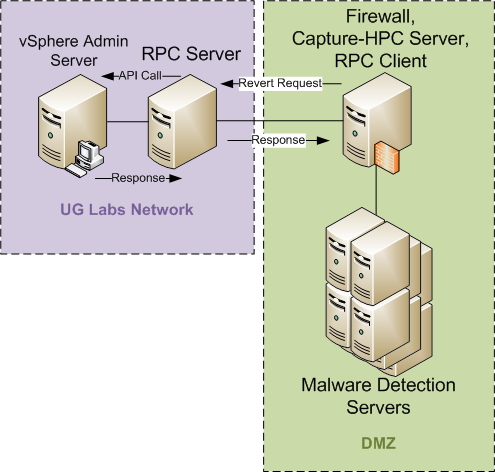
\includegraphics[width=0.8\textwidth]{img/revert-rpc.png}
\caption{Revert RPC Architecture}
\label{fig:revert-1}
\end{figure}

\subsubsection{Framework Integration}

Capture-HPC, being written in a combination of Java, C++ and C needs an
interface module before it can be integrated with the python framework.
Capture-HPC can be backed using a database for URLs, which is useful as it
allows us to build Capture-HPC's database format into a Django ORM which can
be used in the python code to access the database. Due to issues with the
version of Python on the locked-down Red Hat VM, most of the control happens
remotely, aided by the accessibility of the database server on the network. Each
Capture-HPC server has an RPC server and database server on it, which a remote
celery worker can connect to. Once the worker has loaded the URLs into the
database, it starts the Capture-HPC server and waits for the server to finish
processing URLs by periodically checking the database. Once the database
indicates all of the URLs have been scanned, the URLs are deleted from the
database and the RPC server is instructed to terminate the Capture-HPC server.
%TODO: DB stuff might be wrong
The results are returned by the celery worker to the framework for storage in
the framework's result storage database. Tasks for Capture-HPC are routed
specially through the framework, as only explicitly configured workers can
interface with the Capture-HPC server.

\subsubsection{Exclusion Lists}

The exclusion lists used to determine what activity is judged by the Capture-HPC
clients as malicious also needs to be maintained. The Capture-HPC server is
capable of sending the lists to the clients, allowing easy distribution of new
exclusion lists. The exclusion lists as of time of writing are included in
the attached data package, and are stored under the project version control, but the lists
created are only tested with Windows XP, so it is quite possible that they will
need to be modified for use under Windows 7 or Windows Vista.


\subsection{Testing}

Due to the complexity of the Capture-HPC malware scanner, the individual
components that make up the scanner as seen by the framework had to be first
tested individually, and then tested as a single component.

The first unit tests involved running Capture-HPC from the command line, and it
was quickly discovered that some work was needed to get the revert script to
function correctly. After spending a considerable amount of time getting an RPC
mechanism working, it was possible to test Capture-HPC on some URLs. The URLs
used for unit testing consisted a small list of very common websites, and an
executable hosted on an ECS internal server. When configured to detect any
downloaded executable as malware, Capture-HPC correctly identified the
executable file as malware.

The framework integration was unit tested by running the integration script
manually in a django shell, and it was discovered that another RPC comonent was
needed as the version of Python on the gateway was not sufficient. Once the RPC
component had been completed and the integration script proven to work,
Capture-HPC was tested in the full framework, and after revealing a few bugs in
the framework it was successfully running on URL lists. Further testing will
need to be carried out to determine whether the exclusion lists are correct,
with any missing parts coming to light over time as the framework is used.

\subsection{Evaluation}



\clearpage
\section{HTML Analysis Malware Scanner}

HTML Malware Scanner aims to identify the infected HTML webpage. A major problem in designing this scanner is the lack of a clear definition of a malware webpage. Web pages containing illegal content are considered as a malware webpage. Also, the contents of some webpages might appear innocent but some links in those webpages may direct the user to an unauthorised website. The latter is the most popular method attackers use to target internet users. Therefore, finding a solution for this scanner is challenging. Attackers use trendy keywords to increase the probability of a successful attack. In this project, we seek to observe the relationship between the trendy keywords and infected webpage.

\subsection{Design}

The design of the HTML scanner is based upon the frequency of a repeated trendy keyword on a webpage. The HTML scanner accepts two inputs, a URL and a keyword. The scanner searches the webpage to find the quantity of the given keywords. In addition, the scanner identifies all hyperlinks within the given webpage and in turn searches the content of each linked URL to establish the quantity of the given keywords contained within the linked webpages. The frequency of the keywords within the main URL webpage is divided by the sum of frequency of the keywords within the linked webpages in order to calculate a ratio. The HTML scanner used the ratio to decide whether a given URL is malicious or not. Section 12.1 illustrates the implementation of the HTML malware scanner and provides details of this ratio calculation.

Most importantly,there are iteration built into this system, with the HTML scanner also searching the inner URLs and any subsequent hyperlinked web pages. This iteration is carried out until there are more hyperlinks continued within the web page of inner URLs. Hence, the malware writers cannot bypass the scanner by inserting more keywords in the inner hyperlinks. 


\subsection{Implementation}
The fact that there is an unclear definition of a malicious webpage makes the implementation of a malware detection system quite challenging. 	  
	

\subsubsection{Frequency of the keyword}
 
In this approach HTML malware detection takes a URL and a keyword as an input. The HTML crawler scans the main webpage and counts the frequency of the given keyword in that webpage. Also, the crawler scans the contents of the webpage for all the hyperlinks in the main webpage. The scanner then computes the ratio as showed below;

Ratio = Total number of keywords within the main web page / Total number of keywords in the inner hyperlinked web page 

There are three possible ratio result as shown below:
\begin{enumerate}
\item 
$Ratio = 0$\\
The zero ratio indicates the keyword does not exist in the main web page. Therefore the attackers used, a trendy keyword in the components of the given URL to misdirect the user to the malicious webpage. 
\item
$Ratio = infinity$\\
According to the ratio equation, there is no instance of a given keyword within the inner hyperlinked web page. Therefore, the contents of the inner hyperlink web page are not relevant to the content of the main web page. Hence, the given URL is deemed malicious.
\item
$Ratio < 1$\\
That means the number of trendy keyword appears in the main page is more than or equal to the total number of trendy keyword in the web page inner links. In the other words, the contents of the inner links web page is less relevant to the contents of the main web page. In this case the given URL has identified as a malicious URL. 
\item
$0 < Ratio < 1$\\
If the ratio is closer to zero that means the number of keywords appearing in the inner hyperlinked web pages are greater than the number of the keywords on the main web page. Hence, a smaller ratio indicates a higher probability that a given URL is benign. Accordingly, a large ratio (ratios close to one) has a greater probability that the given URL is malicious.
\end{enumerate}
\paragraph{} 
The prima facie weakness of this approach is the risk that a malware writer will insert many instances of trendy keyword terms within the inner hyperlinked web page and instead add malicous hyperlinks from within the inner hyperlinked webpage to another malicious websites or perhaps even from a further removed linked website. Thus, a malware writer could use an iterative process to manipulate the ratio result.To avoid this problem, there is similarly a iterrative process for checking and calculating a ratio at each instance when there are links to another webpage. Hence, the ratio may not inidicate a malicious web page at the first few iterations but then identify a malicious website after checking the last inner hyperlinks. Adapting this method has helped to overcome the major problem for designing HTML malware scanner, because it is independent of the malware definition. In additions, the method is fairly fast.  

\clearpage

\section{ClamAV Malware Scan}
In order to fully identify the existence of malware inside a webpage, a 
signature based malware detection method must be implemented in the system. 
The most obvious approach was to add anti-virus software to the scanning system, 
in order to enable the classification of URLs and files with non-HTML contents, such 
as binary files and scripts. Therefore ClamAV was used as a step in scanning for this purpose, which is also a low interaction malware detection 
method.

\subsection{Design}
\subsubsection{Introduction to ClamAV}
ClamAV is an open source anti-virus software developed for UNIX, and is 
available to Linux systems. It has a command-line scanner with an open access 
signature database, where the anti-virus engine is in a shared library. 
The software provides both on-demand and on-access scanning on Linux systems, 
where on-access scanning is achieved with a scalable multi-threaded daemon. 
It also has wide support for various file formats, including almost all 
popular compressed files, emails and documents. \\
A report in 2011 rated ClamAV 12th among all publicly released anti-virus 
applications,\cite{shandowserver} where the most impressive part is its fast 
response time and scanning speed. This is a key feature that is particularly useful 
because the processing of large URL
datasets requires considerable computing power. \\
ClamAV also has a third party Python API known as pyClamAV. It is a free 
library implemented in C and binds to the ClamAV's own API, libClamAV. However 
the newest version has moved its focus to pyClamd, which is an interface to ClamAV 
daemon instead of libClamAV. Due to the latest updates to ClamAV, some 
key APIs were removed from libClamAV. \\
The conclusion made was to use ClamAV over other 
anti-virus software for the following reasons: 
\begin{itemize}
\item Open source
\item Large signature database and high detection rate
\item Linux compatible
\item Python compatible
\item Wide support for various file types
\item Fast response time and scanning speed
\end{itemize}

\subsubsection{ClamAV with HTML crawler}
A program was built to download URLs and perform static analysis conforming to low interaction. The given URL is expected to contain 
an HTML file, and after the virus scan the program crawls the file in order to extract links to pages 
under the website. After that the extracted links are again downloaded and 
scanned with ClamAV. This time the file types are uncertain, therefore the program is given a max file size to download as well as a time limit in case of a 
slow or broken connection. This is a vital step to avoid downloading huge files such as 
high definition videos as well as those without a file length, for example, a live radio stream.
If the given root page is not an HTML file the program simply scans the file content. 
Links to other domains are ignored because only the investigation 
of the given URL's domain is concerned. More than once links are removed and the 
program avoids downloading the same page twice or more. A root page may need 
to be processed twice: once for crawling and once for virus scan.

Every ClamAV scan is performed by a separate Celery task, which means the 
number of tasks should be $n+1$ where n is the number of interesting links.

\subsection{Implementation}
\subsubsection{Libraries}
The following libraries are used in this Python application:
\begin{itemize}
\item {\bf pyClamd} This is the ClamAV daemon library used for URL content 
scanning. Compared to ordinary ClamAV, a daemon is faster and 
multi-threaded. 

\item {\bf requests} The network library used for HTTP inquiries. In the 
program it is used for downloading the root HTML page as well as the links. 

\item {\bf lxml.html} lxml is a Python XML library. It creates a 
binding to the C libraries libxml2 and libxslt.\cite{lxml} lxml.html is a 
package specifically designed for HTML parsing and acts as an HTML crawler 
which extracts links. 

\item {\bf eventlet.timeout} Eventlet is a Python library that enables 
concurrent networking. The $timeout$ package provides a universal timeout 
solution achieved with green threads, and it is this package that makes the time limit 
for downloads achievable. 
\end{itemize}

\subsubsection{Program implementation}
The program flow is as follows:
\begin{enumerate}
\item A Celery task is created with the crawler function given a URL as a 
parameter. The URL is then downloaded via the \verb`requests` library. 

\item The HTML parser parses the downloaded content as an HTML file, then makes 
all links in it absolute.

\item All links are extracted with the library function {\em html.iterlinks()} and
results are returned as a list for easy manipulation. Duplicate links and 
those with different domain names are removed.

\item For each link the download function is called with a separate Celery 
task. A get request which only acquires HTTP headers is sent, such that the file size can be determined by the 
{\em content-length} field. If the file length is within a pre-defined limit, just before 
the download begins a green thread with a {\em Timeout} is created which throws 
an exception if the download time is too great. Zero is returned if any exception 
occurs before or during downloading. Exceptions include but are not limited to request 
exceptions (such as error response code) and time outs. After successful 
downloading a clamd scan to the content is called, and the return value should be 
either {\em None} or the virus description message. 

\item The final list of malware detected is merged with the results 
returned from the scan results of all downloaded links as well as those from the root 
page, this then returns to the main system.  
\end{enumerate}

\subsection{Testing}
The program's individual functions were tested separately. The sequence of 
testing was as following:
\begin{enumerate}
\item Downloading and parsing of HTML.
\item Extraction of links and make them absolute.
This was tested by printing all links as absolute from a given HTML and checking 
manually.
\item Removal of duplicate links and those links to other domains.
\item Downloading of an arbitrary URL.
This function was tested by downloading testing websites such as
\verb`http://www.thinkbroadband.com/download/`
The tests with various file 
sizes passed without errors and those links that exceeded the size or time limits were 
ignored. 
\item Clamd scan of the downloaded contents. 
\end{enumerate}
\paragraph{}
After that the whole program was tested with benign websites which provide 
testing for various viruses. These files used for testing were not real viruses however anti-virus packages recognize these signatures 
as part of their test suite. 
One of the websites used was Eicar\cite{eicar}. This website provides a small test 
virus in three compressed levels: plain text, zipped and double-zipped, with 
download links in the same page. The results obtained after 
crawling the web page are presented below:
\begin{verbatim}
[('http://www.rexswain.com/eicar.com', 
{'stream': ('FOUND', 'Eicar-Test-Signature')}), 
('http://www.rexswain.com/eicar.zip', 
{'stream': ('FOUND', 'Eicar-Test-Signature')}), 
('http://www.rexswain.com/eicar2.zip', 
{'stream': ('FOUND', 'Eicar-Test-Signature')})]
\end{verbatim}
Consequently the unit testing of the ClamAV scanner was successful. 

\subsection{Evaluation}



\clearpage
\section{High interaction malware detection with Wine}
\subsection{Design}
This section details one of the high interaction malware detection 
approaches used in the system. The major 
feature of this approach is capability to detect unknown malicious 
actions. This project has a system called Wine Explorer, 
which is typical of a high interaction approach. It uses Wine as a compatibility layer to run 
Internet Explorer 6 in a Linux environment and is capable of scanning for 
possible file operations performed by malicious websites. 

\subsubsection{Wine Is Not an Emulator}
Wine is a widely used free software which acts as a compatibility layer 
capable of running Windows applications on non-Windows operating 
systems.\cite{wikiwine} It is unlike virtual machines and emulators which simulate 
internal Windows logic, ``Wine translates Windows API calls into POSIX calls 
on-the-fly, eliminating the performance and memory penalties of other methods 
and allowing you to cleanly integrate Windows applications into your 
desktop.''\cite{aboutwine} Originally a ``backcronym'' WINE stood for ``Wine Is Not an 
Emulator''. Wine is able to run most Windows applications 
without any performance drop as long as there are no performance related bugs, 
especially for 2D applications. Whilst Wine is an 
extra layer on the top of the system, there is no difference to programs that 
uses extra libraries. An example of such software is the compatibility 
mode in newer versions of Windows designed for running legacy 
software.\cite{wineperformance}
\paragraph{}
Wine has advantages over conventional virtual machines particularly in terms 
of working with web browsers. Although 
virtual machines have advantages in simulating programs which give more 
realistic environments, they use additional resources. In most cases, a 
virtual machine consumes significantly more memory, disk space and CPU, as it 
needs to simulate the whole operating system instead of a providing a layer 
to a program. Wine treats Windows applications as ``first-class citizens'', 
which run at full speed.\cite{wineperformance}
\paragraph{}
Wine uses a working directory as a complete Windows system which stores all 
information about the specific system's configurations and files in its virtual 
hard drive. The active working directory is known as the Wine prefix. 
One of the discoveries in Wine is that the creation of Wine prefix is 
lightweight and resource saving compared to that of a virtual machine or
emulator. The Wine prefix itself also conforms to the nature of a 
sandbox. This means almost all kind of behaviours performed 
by programs inside the Wine prefix cannot affect the underlying system. 
A potential threat is the unrestricted permissions 
for applications in Wine prefix, which by default exposes the root file 
system to them, however malwares running in Windows that manipulate Linux 
file systems are rather rare. \\
The conclusion is that Wine is a suitable 
tool for creating a client honeypot in high interaction malware detection. 

\subsubsection{Execution Flow}
Wine Explorer is a straightforward program, and Figure \ref{fig:wine}
illustrates the execution flow of detecting a single URL. \\
\begin{figure}[htb]
\centering
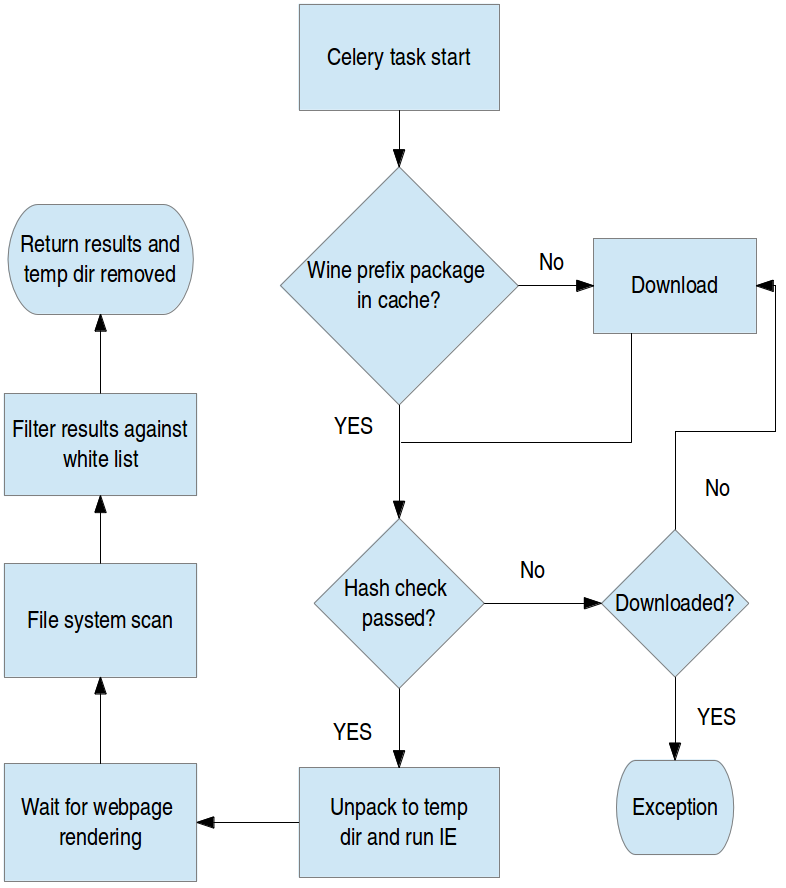
\includegraphics[width=0.8\textwidth]{img/wine-flowchart.png}
\caption{Program flow}
\label{fig:wine}
\end{figure}
With Wine Explorer, URLs given by the URL classifier are opened with the specific instance of Internet Explorer inside the Wine 
prefix. 
These URLs are said to be strongly suspicious of containing malware and are 
supposed to be investigated in depth. \\
In order to speed up Wine prefix creation, a clean Wine prefix packed with 
Internet Explorer 6 is prepared. Therefore whenever a new Wine prefix is needed, 
the only process is to unpack it to a desired location. 
The package's SHA-256 hash is calculated and stored in Wine Explorer so that 
its validity can be ensured. 
The package is then uploaded into a web drive and can be downloaded in 
order to increase the system's portability. \\
The system should also be able to store multiple instances of Wine prefixes 
and execute Internet Explorers in them concurrently. 
After an execution is completed a scan is performed to check file system 
modifications inside that Wine prefix. 
A white list is provided which describes files which might be modified by
system operations. 
The results are then returned to the main system, and the temporary Wine 
prefixes after scanning should be removed in order to save disk space. 

\subsection{Implementation}
Python is used to implement this program just as other parts of this project. 
WineBrowser, an instance of Wine prefix running it, manages all operations 
with a single URL. Details on how the program work are as follows:
\begin{enumerate}
\item \verb`create_wine_prefix(template_spec)` \\
Check cache for the package containing the predefined Wine prefix. If it does
not exist, download it, and perform a hash check.
If success the package is unpacked to a temporary directory. 
\item \verb`WineBrowser.__init__()` and \verb`WineBrowser.run()`\\
The active Wine prefix is set to the temporary directory, and the Internet 
Explorer is run with the given URL under Wine. 
\item
Wait for 30 seconds.
\item \verb`check_change(dir1,dir2)`\\
Check the file system changes. This is achieved by running {\em filecmp} recursively 
for all files between the clean Wine prefix and the active one. The results 
are filtered against a white list then returned to the main system. The white 
list is included in the appendix.%TODO 
\item \verb`WineBrowser.close()`\\
Remove the temporary directory. 
\end{enumerate}
Any web pages take more than 30 seconds to 
load will be discarded as one will significantly lower the system's 
throughput. \\
The main system runs one WineBrowser instance with Celery per task, in order 
to achieve concurrent execution of multiple Wine programs at the same time increases the overall throughput dramatically. 

\subsection{Testing}
After the first draft of implementation of the Wine Explorer, its functions are
tested individually before combine to a whole module for unit testing. This is a sample 
output from \verb'check_change' when comparing a modified Wine prefix with 
the clean one:
\begin{verbatim}
(['wineprefix_ie6', 'user.reg~'], 
['winetricks.log'], 
['user.reg'], 
[])
\end{verbatim}
Each array in the record stores newly created files, removed files, 
modified files and files the system is unable to check respectively. 
\paragraph{}
In conclusion, all functions 
explained in the implementation section are ensured to work separately, 
however the websites that affect file systems are yet to be found. 
This program will be further polished when we produce a demo 
of the whole project in the future. 




\subsection{Evaluation}





%END INCLUDED TECH SECTIONS

\nomenclature{SSL}{Secure Sockets Layer}
\nomenclature{HTTP}{Hypertext Transfer Protocol}
\nomenclature{REST}{Representational state transfer architecture}




%
\subsection{Implementation}
The fact that there is an unclear definition of a malicious webpage makes the implementation of a malware detection system quite challenging. 	  
	

\subsubsection{Frequency of the keyword}
 
In this approach HTML malware detection takes a URL and a keyword as an input. The HTML crawler scans the main webpage and counts the frequency of the given keyword in that webpage. Also, the crawler scans the contents of the webpage for all the hyperlinks in the main webpage. The scanner then computes the ratio as showed below;

Ratio = Total number of keywords within the main web page / Total number of keywords in the inner hyperlinked web page 

There are three possible ratio result as shown below:
\begin{enumerate}
\item 
$Ratio = 0$\\
The zero ratio indicates the keyword does not exist in the main web page. Therefore the attackers used, a trendy keyword in the components of the given URL to misdirect the user to the malicious webpage. 
\item
$Ratio = infinity$\\
According to the ratio equation, there is no instance of a given keyword within the inner hyperlinked web page. Therefore, the contents of the inner hyperlink web page are not relevant to the content of the main web page. Hence, the given URL is deemed malicious.
\item
$Ratio < 1$\\
That means the number of trendy keyword appears in the main page is more than or equal to the total number of trendy keyword in the web page inner links. In the other words, the contents of the inner links web page is less relevant to the contents of the main web page. In this case the given URL has identified as a malicious URL. 
\item
$0 < Ratio < 1$\\
If the ratio is closer to zero that means the number of keywords appearing in the inner hyperlinked web pages are greater than the number of the keywords on the main web page. Hence, a smaller ratio indicates a higher probability that a given URL is benign. Accordingly, a large ratio (ratios close to one) has a greater probability that the given URL is malicious.
\end{enumerate}
\paragraph{} 
The prima facie weakness of this approach is the risk that a malware writer will insert many instances of trendy keyword terms within the inner hyperlinked web page and instead add malicous hyperlinks from within the inner hyperlinked webpage to another malicious websites or perhaps even from a further removed linked website. Thus, a malware writer could use an iterative process to manipulate the ratio result.To avoid this problem, there is similarly a iterrative process for checking and calculating a ratio at each instance when there are links to another webpage. Hence, the ratio may not inidicate a malicious web page at the first few iterations but then identify a malicious website after checking the last inner hyperlinks. Adapting this method has helped to overcome the major problem for designing HTML malware scanner, because it is independent of the malware definition. In additions, the method is fairly fast.  

%\subsection{Testing}
The program's individual functions were tested separately. The sequence of 
testing was as following:
\begin{enumerate}
\item Downloading and parsing of HTML.
\item Extraction of links and make them absolute.
This was tested by printing all links as absolute from a given HTML and checking 
manually.
\item Removal of duplicate links and those links to other domains.
\item Downloading of an arbitrary URL.
This function was tested by downloading testing websites such as
\verb`http://www.thinkbroadband.com/download/`
The tests with various file 
sizes passed without errors and those links that exceeded the size or time limits were 
ignored. 
\item Clamd scan of the downloaded contents. 
\end{enumerate}
\paragraph{}
After that the whole program was tested with benign websites which provide 
testing for various viruses. These files used for testing were not real viruses however anti-virus packages recognize these signatures 
as part of their test suite. 
One of the websites used was Eicar\cite{eicar}. This website provides a small test 
virus in three compressed levels: plain text, zipped and double-zipped, with 
download links in the same page. The results obtained after 
crawling the web page are presented below:
\begin{verbatim}
[('http://www.rexswain.com/eicar.com', 
{'stream': ('FOUND', 'Eicar-Test-Signature')}), 
('http://www.rexswain.com/eicar.zip', 
{'stream': ('FOUND', 'Eicar-Test-Signature')}), 
('http://www.rexswain.com/eicar2.zip', 
{'stream': ('FOUND', 'Eicar-Test-Signature')})]
\end{verbatim}
Consequently the unit testing of the ClamAV scanner was successful. 

%Evaluation, Project Management Summary (gantt comparison etc.)
\subsection{Evaluation of ClamAV Malware Scan}
Anti-virus scanning gives the system the ability to detect malicious 
signature patterns in various file types that may exist in webpages. The 
testing results proved the fast response and scanning speed of ClamAV. The 
program returns an list of malware found in a particular website and 
is self-contained.

A limitation 
of this project is the exclusion of links to other domains. It might be too 
decisive which is highly possible to miss malicious files, as it is 
not rare to see a webpage contain a direct download link which points to a 
virus executable hosted on another website that cannot be easily found by 
a search engine. Apart from other disadvantages inherited from a low interaction 
detection method, the system does not filter obvious 
harmless file types, such as images and videos. It could have been a more polished system if 
the project schedule was more flexible.


\subsection{Project Management Summary}

\subsubsection{Time Management Record}

To effectively manage time over the course of the project the group constructed
a gannt chart to track the components tasks of the project and to fit those tasks into the
tight schedule defined by the project guidelines. To build the gantt chart the
group first plotted the milestones of the project (shown as diamonds on the
gantt chart); submitting a brief to the
customer, the two progress seminars, the report hand-in and the final
presentation. The time between the milestones formed the development cycles
used in the project, with two iterations of development of four weeks in length
each before each progress seminar. One week at the end of each iteration was
left for preparation of the progress seminar.

At the end of the first iteration, the group was on time with the deliverables
set in the plan, and there was time during the preparation of the first progress
seminar to integrate the code produced and present a demo of the framework
retrieving trends and URLs. After the progress seminar the group started to work on
the malware scanners, having researched scanning methods during the first
iteration. When preparing for the second progress seminar, the group started to
suspect that the task of creating and integrating malware scanners into the
framework was harder than originally estimated, resulting in development effort
continuing after the second progress seminar in contrast to the plan. The
consequence of this was reduction in scope for the amount of results
collected, and the delay of the web reporting interface to an additional task
completed after the delivery of the rest of the project but still in time for
presenting to the customer at the final presentation.

The Gantt charts can be found in Appendix B.

\subsubsection{Writing the Report}

Although the first words of the report were written in early November, writing
the report started in earnest at the beginning of December. To aid the group
with assessing current progress with the report, a python script was written
that shows a day by day cumulative word count drawn on a stacked bar chart with
one segment per group member. The output of the python script is shown in Figure
\ref{fig:rep-1}.
This script uses the github API and texcount.pl script to count words in each
commit in the repository.

\begin{figure}[htb]
\centering
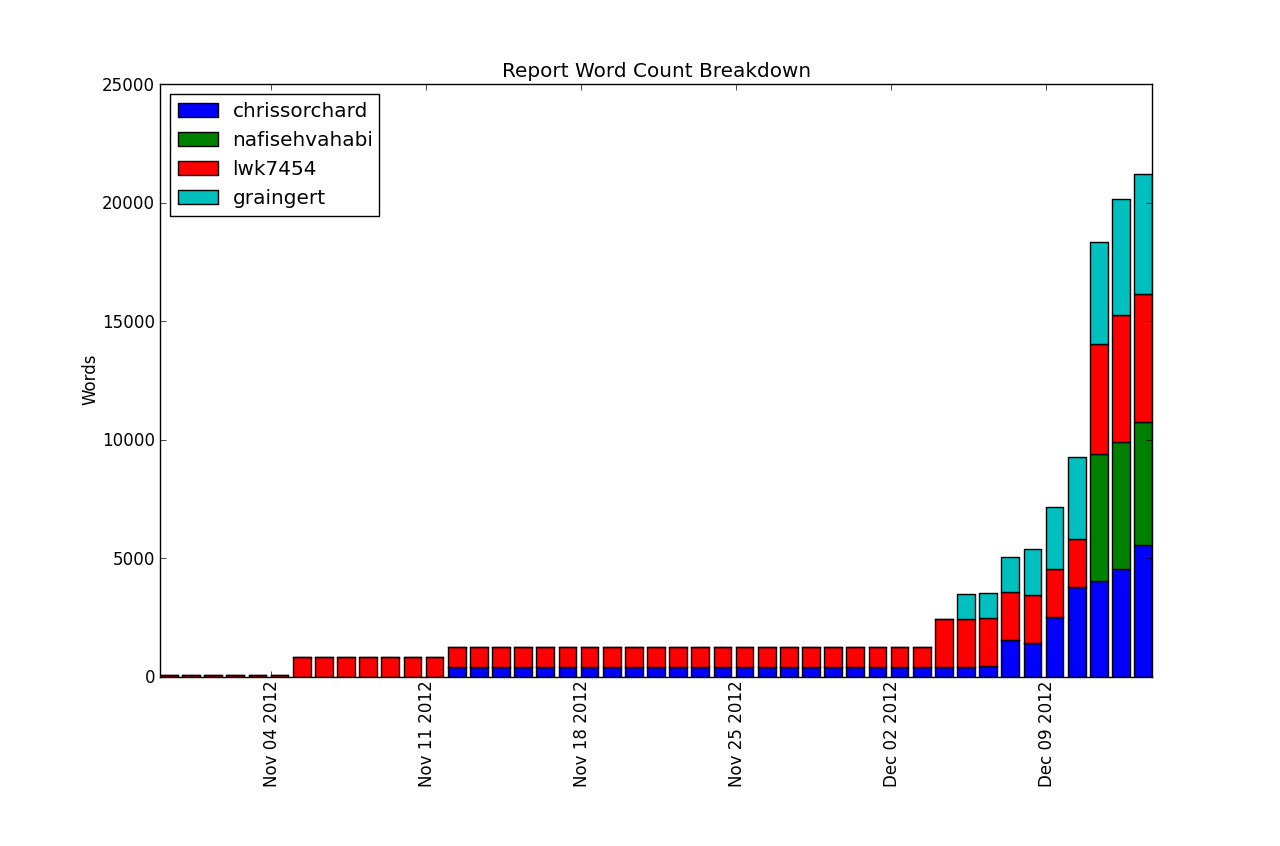
\includegraphics[width=0.8\textwidth]{img/reportificate.png}
\caption{Final Report Word Count Breakdown}
\label{fig:rep-1}
\end{figure}

Sections of the report were allocated to group members using a spreadsheet that
can be found in the accompanying data package under
\verb`doc/tools/word-org.ods`. The spreadsheet provided useful validation for
the sum of words allocated, and ensured that group members were not given an
unfair amount of report to write.

\subsubsection{Achievements \& Lessons Learnt}

The total length of time available to complete the project in was 11 weeks, in
this time the group had to fit in a customer brief, two presentations, and a
24000 word report. This meant that the effective development time for the
project was in the region of 4-6 weeks. In this time the group managed to
construct a working framework that could collect trends from a number of
sources, retrieve URLs related to those trends, and conduct rudimentary analysis
of the URLs for malware. As of writing the only working malware scanners are
those which involve the very lowest levels of interaction. Whilst the
Capture-HPC scanner was successfully integrated into the framework, further
configuration of the system is needed before it can be used to process URLs in
an effective way. The other malware scanners are not yet fully integrated into
the framework. Given the time constraints, the group managed to achieve most of
the work needed for a fully featured prototype and it is expected that it will be
possible to demo a completed version of the project at the final presentation to
the customer. In retrospect the scope of the project was very wide, and perhaps
a more complete product could have been delivered if the scope had been reduced
somewhat.

Another lesson learned during the course of the project relates to the division
of work. The style of development was intended to allow a reasonable degree of
autonomy, but still provide ample opportunity for the group members to assist
each other with tasks in case of difficulty. An unintended consequence of this
was that no one group member had complete knowledge of all of the technical
aspects of the system, making integration more complicated and hence causing
delays.


%Conclusions + future work
\section{Conclusion} 
\subsection{URL Classification}

%need to make sure it is clear that we're talking about the URLs rather than the content?
An unknown malicious URL cannot be identified by systems that use signature-based malware detection methods. As a solution, the designed system includes a classifier in order to detect unknown malicious URLs. The classifier relies on pattern matching algorithm used in the Levenshtien distance and has two classes of data; malicious URLs and clean URLs. An unknown URL enterings to the detection system will be classified based on its similarity to the URLs in the dataset. The result of the classification algorithm provides a confidence rate regarding the URL’s maliciousness. Depending on the confidence rate provided, the classifier will then classify whether the given URL should be subject to a heavyweight or lightweight scanning process. However, where the URL is already held within the database, an immediate result is returned confirming with a one hundred percent confidence rate whether or not the URL is malicious. Because a given URL does not need to be checked by multiple scanners simultaneously and unnecessarily, the classifier creates a more efficient and robust detection system. 
 
\subsection{HTML Scanning}

The HTML malware scanner specifically processes trendy keywords from a search engine and within an infected web page to detect a malicious URL. The HTML scanner has been designed based on the repetitive frequency of the trendy keywords within the main URL web page and within the contents of associated hyperlinked web pages. The scanner is efficient and can easily be extended with sophisticated techniques to produce more accurate results. 
 
\subsection{Wine Explorer and ClamAV scanner}
Wine Explorer provides a lightweight solution for high interaction malware 
detection. It has advantages over virtual machines and emulators including 
short reset time, fast execution and RAM/disk saving, where the potential 
security threat blocks its way to perfection. The program is also approved to 
execute stably, for instance the correctness of the Wine prefix package is 
guaranteed via hash check which avoids external modifications of it. The group 
explained the lacking of complete detection as well, which could be 
implemented if we had more time in this project. 
\paragraph{}
The group also provide a signiture-based malware scanning program powered by ClamAV. 
The 
HTML crawler in the same program gives links for ClamAV to scan and an 
overall list of malicious links in a webpage can be produced at last. 
It has fast scanning and concurrent execution features which rises 
the system's throughput to a significant amount. However disadvantages still 
exists, 
such as unprecise link filtering. An improvement could be a deeper level of 
website crawling or better link processing which requires further amount 
of time to complete. 


\subsection{Capture-HPC}

Capture-HPC is a high interaction client honeypot, a system designed to actively
search for malware by rendering the content at provided URLs. In addition to
offering a accurate simulation of a user browsing the web Capture-HPC provide
much flexibility, capable of automatically rendering content using a variety of
client programs including web browsers such as Internet Explorer and Firefox,
and the PDF viewer Adobe Reader. It also allows a degree of freedom in choosing
the sensitivity of the malware detection using the exclusion lists, a feature
that also makes the process of porting Capture-HPC to other Windows OSs
considerably simpler.

Capture-HPC was found to be fairly slow, justifiable by the amount of work that
must happen to render the content in a real web browser. The issue of speed
meant that Capture-HPC has been integrated into the framework with some care,
restricting the number of URLs passed to it via classification to attempt to
limit the execution time for a set of URLs. Despite this Capture-HPC still 
remains one of the more powerful malware scanners available in the framework.

\subsection{Framework}

Using a distributed framework as a foundation for the project proved successful,
although issues arising from the complexity of adapting code to run on the
framework detracted somewhat from its effectiveness. The framework as
implemented using Celery, RabbitMQ and Redis was capable of effectively
distributing tasks to workers using routing features provided to route specific
tasks to a specific worker, needed by the Capture-HPC malware scanner which
requires configuration and resources outside of the scope of the framework.
Caching was also effectively used to reduce duplicate requests, with most of the
workers implementing Redis caching of URLs mapped to results.

\subsection{Project Conclusions}

Unfortunately, the project did not sufficiently progress to test the hypothesis:
is malware specifically targeted at trending topics. This would have required
considerable time to collect data, and the reliability of the project in
classifying URLs as malicious or benign has not yet been determined as this is a
property of the combination of malware scanners used and confidence ratings
applied to the scanners. A small suite of scanners has been assembled and
tested, including web lists and Capture-HPC.

The project has successfully combined distributed task framework with trend
sources, search retrieval, and malware scanning and the end result is a
re-usable framework appropriate for carrying out further investigation into th
hypothesis. It is hoped that some data collected and a preliminary conclusion to
the hypothesis can be found in time for the final presentation to the customer.
 

\section{Future development}

The main weakness of the classier in its current form is its processing speed. With the aid of the machine learning algorithm, the speed of the URL classification can be improved. At the moment, the pattern-matching algorithm needs to match a given URL with every single URL in the URL database, which containing both malicious and benign URLs. Malicious and benign URLs can be converted into the form of a vector. These two vectors allow additional machine learning methods such as Support Vector Machine (SVM) or Multi-Layers Perceptron (MLP) to be applied. This reduces the need for matching a given URL to every single URL within the URL database. However, converting the URL to a form of a vector is very challenging in terms of implementation effort because the structure of a URL does not have a repetitive pattern.

\paragraph{}
The second development for the classifier is to use different classification algorithms and then to compare and contrasts their performance. Three machine learning technique algorithms are suggested for implementation, namely; Naïve Bayes, Support Vector Machine (SVM) and Decision Tree. The implementation of these three algorithms requires two datasets; a training and a testing dataset. A list of URLs can be used as training dataset for the classifier and a separate list of URLs is required for the testing dataset. URLs in the testing dataset should be completely different from those URLs in the training dataset. The important aspect involves the selection of URL features for classification. Many features can be considered such as; length of the URL, number of forward slashes '/'or the number of dots '.'' used in the URL structure. Features extracted from the URL’s structure are used as input for the classifier. The classifier will use extracted features to distinguish a malicious URL from the benign URL. 

\paragraph{}
In the current system the HTML malware scanner uses a URL and a keyword as the input and based on the frequency of the keyword in the web page of the given URL decides whether the URL is malicious or clean. An alternative design for the HTML scanner involves continuously updating a database with a feed of new trendy keywords so that the HTML scanner’s only input requirement is a given URL. The challenging part of this model is designing of a trendy keyword database, with each trendy keyword belonging to a group of keywords that have the same topic. The database will be connected to a list of selected trusted website such as BBC News. In turn, the database can be updated with any new trendy keywords being used on the News website, with old keywords being removed from the database after a predefined time period e.g. one month. In this model, the scanner decision is not only based on one trendy-keyword, it is based on a group of keywords connected to the trendy keyword topic within the database. Hence, ensuring a more reliable result is provided by the malware scanner.

\paragraph{}
Another option for the design of the HTML malware scanner involves considering the features of the web page related to each URL. In this method, a list of features of the webpage is extracted. This method is very similar to the one already suggested for the classifier. Again, there is a list of training dataset and testing dataset for the classifier, but instead the extracted features from web page will used as an input for the classifier. The web page features may be the number of hyperlinks in the webpage, number of lines, word count and functions (JavaScript keywords).

After training the classifier, some features may provide more useful results such as the use of JavaScript function in the web page. Hence, the features that produce the most accurate results will be selected for classification. Although the latter model does not consider the relationship between the trendy keyword term and the malicious URLs, a powerful system with an updated database and classifier can be created by combining the above two models. As a result, the database would contain a list of trendy keyword terms updated from trusted websites and the classifier would be capable of identifying unknown malicious URLs relating to the trendy keyword term.

The malware detection system that employs machine-learning techniques has a few advantages. The system can overcome the problem of detecting an unknown malware and also polymorphic malwares. In addition, it is very efficient and resilient in comparison with other malware detection techniques. Moreover, the adapted techniques in this system make it difficult for malware writers to bypass the detection system. 









%references
\addcontentsline{toc}{section}{References}
\bibliographystyle{IEEEtran}
\bibliography{final-report,rfc,i-d,tag1g09,cso1g09,nv2g09,wl15g09}{}

%Appendices
\appendix
\verbatiminput{appendix/foo.txt}
\section{List of Abbreviations}
\renewcommand{\nomname}{}
\printnomenclature

\clearpage

\section{RADIUS configuration}
\label{sec:Code;sub:radius}

\subsection{/etc/raddb/users}
\begin{verbatim}[frame=single]
#Give access to this user
TomB    Cleartext-Password := "TomBsPassword"
        Reply-Message = "Hello there %{User-Name}! How's it going?"

#Don't give access to this user
TomG    Auth-Type := Reject
        Reply-Message = "Oh no you don't Grainger. Not again."
\end{verbatim}

\subsection{/etc/raddb/clients.conf}
\begin{verbatim}[frame=single]
client linuxproj {
    ipaddr = 152.78.71.57
    secret = testing123
    require_message_authenticator = no
    
    #Used to specify a specific Network Access Server type
    #(e.g. cisco, multitech, etc.)
    nastype = other
}
\end{verbatim}

\subsection{/etc/raddb/eap.conf}
\begin{verbatim}[frame=single]
tls {
    certdir = ${confdir}/certs
    cadir = ${confdir}/certs
    private_key_password = whatever
    private_key_file = ${certdir}/server.pem
    certificate_file = ${certdir}/server.pem
    CA_file = ${cadir}/ca.pem
    dh_file = ${certdir}/dh
    random_file = ${certdir}/random
    CA_path = ${cadir}
    cipher_list = "DEFAULT"
}

ttls {
    default_eap_type = md5
    copy_request_to_tunnel = no
    use_tunneled_reply = no
    virtual_server = "inner-tunnel"
}
\end{verbatim}

\section{Authenticator}
\label{sec:Code;sub:authenticator}

\subsection{/etc/hostapd/hostapd.conf}
\subsubsection{802.1X}
%TODO: add stuff

\subsubsection{802.11r}
\begin{figure}[h!]
\begin{verbatim}[frame=single]
auth_server_addr=152.78.61.5
auth_server_port=1812
auth_server_shared_secret=testing123
disable_pmksa_caching=1
okc=0
nas_identifier=kanga-cso1g09e
eapol_key_index_workaround=1
ieee8021x=1
wpa_key_mgmt=FT-EAP WPA-EAP
auth_algs=1
wpa=2
wpa_pairwise=CCMP
ssid=notthebees
bridge=br-lan
wmm_enabled=1
bssid=00:18:0a:01:3f:38
ignore_broadcast_ssid=0
mobility_domain=a1b2
r0_key_lifetime=100000
r1_key_holder=000102030406
reassociation_deadline=1000
r0kh=00:18:0a:01:3f:3f kanga-cso1g09e
    000102030405060708090a0b0c0d0e0f
r1kh=00:18:0a:01:3f:3f 00:01:02:03:04:05
    000102030405060708090a0b0c0d0e0f
r1kh=00:18:0a:01:3f:38 00:01:02:03:04:06
    000102030405060708090a0b0c0d0e0e
\end{verbatim}
\caption{Configuration by Chris Orchard}
\end{figure}

\section{Supplicant}
\label{sec:Code;sub:supplicant}

\subsection{/etc/wpa\_supplicant/wpa\_supplicant.conf}
\subsubsection{802.1X}
\begin{figure}[h!]
\begin{verbatim}[frame=single]
ctrl_interface=/var/run/wpa_supplicant
eapol_version=1
ap_scan=1
fast_reauth=1

network={
        ssid="notthebees"
        scan_ssid=1
        key_mgmt=WPA-EAP
        pairwise=CCMP
        group=CCMP
        eap=TTLS
        identity="TomB"
        anonymous_identity="anon"
        password="TomBsPassword"
        phase2="auth=PAP"
}
\end{verbatim}
\end{figure}

\subsubsection{802.11r}
\begin{figure}[h!]
\begin{verbatim}[frame=single]
ctrl_interface=/var/run/wpa_supplicant
eapol_version=1
ap_scan=1
fast_reauth=1

network={
        ssid="notthebees"
        scan_ssid=1
        key_mgmt=FT-EAP WPA-EAP
        pairwise=CCMP
        group=CCMP
        eap=TTLS
        identity="TomB"
        anonymous_identity="anon"
        password="TomBsPassword"
        phase2="auth=PAP"
}
\end{verbatim}
\end{figure}

\newpage
\section{Testing Output}

\subsection{Simulation}
\label{sec:testing-output;sub:simulation}

\subsection{wpa\_supplicant output}
\subsubsection{802.1X}
\label{sec:testing-output;sub:supplicant}
\begin{figure}[h!]
\begin{verbatim}[frame=single]
<3>SME: Trying to authenticate with 00:18:0a:01:3f:38
    (SSID='notthebees' freq=2412 MHz)
<3>Trying to associate with 00:18:0a:01:3f:38
    (SSID='notthebees' freq=2412 MHz)
<3>SME: Trying to authenticate with 00:18:0a:01:3f:3f
    (SSID='notthebees' freq=2462 MHz)
<3>Trying to associate with 00:18:0a:01:3f:3f
    (SSID='notthebees' freq=2462 MHz)
<3>Associated with 00:18:0a:01:3f:3f
<3>CTRL-EVENT-EAP-STARTED EAP authentication started
...
<3>CTRL-EVENT-EAP-SUCCESS EAP authentication completed successfully
<3>WPA: Key negotiation completed with 00:18:0a:01:3f:3f
    [PTK=CCMP GTK=CCMP]
<3>CTRL-EVENT-CONNECTED - Connection to 00:18:0a:01:3f:3f
    completed (reauth) [id=0 id_str=]
> roam 00:18:0a:01:3f:38
OK
<3>SME: Trying to authenticate with 00:18:0a:01:3f:38
    (SSID='notthebees' freq=2412 MHz)
<3>Trying to associate with 00:18:0a:01:3f:38
    (SSID='notthebees' freq=2412 MHz)
<3>Associated with 00:18:0a:01:3f:38
<3>CTRL-EVENT-EAP-STARTED EAP authentication started
...
<3>CTRL-EVENT-EAP-SUCCESS EAP authentication
    completed successfully
<3>WPA: Key negotiation completed with 00:18:0a:01:3f:38
    [PTK=CCMP GTK=CCMP]
<3>CTRL-EVENT-CONNECTED - Connection to 00:18:0a:01:3f:38
    completed (reauth) [id=0 id_str=]
\end{verbatim}
\end{figure}

\subsubsection{802.11r}
\label{sec:testing-output;sub:80211r}
\begin{figure}[h!]
\begin{verbatim}[frame=single]
wlan0: Trying to associate with 00:18:0a:01:3f:38
    (SSID='notthebees' freq=2412 MHz)
FT: Invalid group cipher (0)
wlan0: Authentication with 00:18:0a:01:3f:38 timed out.
wlan0: Trying to associate with 00:18:0a:01:3f:3f
    (SSID='notthebees' freq=2462 MHz)
wlan0: Authentication with 00:18:0a:01:3f:3f timed out.
wlan0: Trying to associate with 00:18:0a:01:3f:3f
    (SSID='notthebees' freq=2462 MHz)
wlan0: Authentication with 00:18:0a:01:3f:3f timed out.
wlan0: Trying to associate with 00:18:0a:01:3f:38
    (SSID='notthebees' freq=2412 MHz)
^Cwlan0: CTRL-EVENT-TERMINATING - signal 2 received
\end{verbatim}
\end{figure}


%TODO: following sections:
%       project description
%       literature review
%       design + spec.
%       justification of approact
%       project control: past, future
%       gantt chart


\end{document}
